%%%%%%%%%%%%%%%%%%%%%%% file template.tex %%%%%%%%%%%%%%%%%%%%%%%%%
%
% This is a general template file for the LaTeX package SVJour3
% for Springer journals.          Springer Heidelberg 2010/09/16
%
% Copy it to a new file with a new name and use it as the basis
% for your article. Delete % signs as needed.
%
% This template includes a few options for different layouts and
% content for various journals. Please consult a previous issue of
% your journal as needed.
%
%%%%%%%%%%%%%%%%%%%%%%%%%%%%%%%%%%%%%%%%%%%%%%%%%%%%%%%%%%%%%%%%%%%
%
% First comes an example EPS file -- just ignore it and
% proceed on the \documentclass line
% your LaTeX will extract the file if required
\begin{filecontents*}{example.eps}
%!PS-Adobe-3.0 EPSF-3.0
%%BoundingBox: 19 19 221 221
%%CreationDate: Mon Sep 29 1997
%%Creator: programmed by hand (JK)
%%EndComments
gsave
newpath
  20 20 moveto
  20 220 lineto
  220 220 lineto
  220 20 lineto
closepath
2 setlinewidth
gsave
  .4 setgray fill
grestore
stroke
grestore
\end{filecontents*}
%
\RequirePackage{fix-cm}
%
%\documentclass{svjour3}                     % onecolumn (standard format)
%\documentclass[smallcondensed]{svjour3}     % onecolumn (ditto)
\documentclass[smallextended]{svjour3}       % onecolumn (second format)
%\documentclass[twocolumn]{svjour3}          % twocolumn
%

\smartqed  % flush right qed marks, e.g. at end of proof
%
\usepackage[pdftex]{graphicx}
%
% \usepackage{mathptmx}      % use Times fonts if available on your TeX system
%
% insert here the call for the packages your document requires

% makes "C++" take up a little less space; man, those plus signs are big
\usepackage{relsize}
\newcommand{\Cpp}{{C\raisebox{0.2ex}{\ensuremath{\mathsmaller{++}}}}\xspace}
\usepackage{paralist}
\usepackage{color}
\usepackage{fancybox}
\usepackage{url}
\usepackage{listings}
\usepackage{fmtcount}
\usepackage[margin=10pt,font=small,labelfont=bf,labelsep=endash]{caption}
\usepackage{float}
\usepackage{comment}
\restylefloat{figure}

\usepackage{amssymb}
\usepackage{ifthen}
\usepackage{xspace}

\makeatletter

\def\ie{\textit{i.e.},\xspace}
\def\eg{\textit{e.g.},\xspace}


\newcommand{\COMMENT}[1]{}
\newcommand{\ndef}{\stackrel{\rm def}{=}}
\newcommand{\minitab}[2][l]{\begin{tabular}{#1}#2\end{tabular}}


\newboolean{showcomments}

\setboolean{showcomments}{true}

\ifthenelse{\boolean{showcomments}}
  {\newcommand{\nb}[2]{
    \fbox{\bfseries\sffamily\scriptsize#1}
    {\sf\small$\blacktriangleright$\textit{#2}$\blacktriangleleft$}
   }
   \newcommand{\cvsversion}{\emph{\scriptsize$-$Id: macro.tex,v 1.9 2005/12/09 22:38:33 max Exp $}}
  }
  {\newcommand{\nb}[2]{}
   \newcommand{\cvsversion}{}
  }

\newcommand\DANIEL[1]{\nb{Daniel}{#1}}
\newcommand\DMG[1]{\nb{DMG}{#1}}
\newcommand\MAX[1]{\nb{Max}{#1}}
\newcommand\JWD[1]{\nb{JULIUS}{#1}}


\newcommand\NEW[1]{\nb{NEW}{#1}}

\newcommand{\varname}[1]{{\small\texttt{#1}}\xspace}


\newenvironment{entry}%
{\begin{list}{}{\noindent
\renewcommand{\makelabel}[1]{\textbf{##1:}\hfil}%
\setlength{\leftmargin}{1.5em}%
\setlength{\itemindent}{1em}%
}}%
{\end{list}}

\newenvironment{hassanbox}%
{\vspace{1mm}\noindent\begin{Sbox}\begin{minipage}{0.97\columnwidth}}%
{\end{minipage}\end{Sbox}\fbox{\TheSbox}}

%% adds by migod
\definecolor{darkgreen}{RGB}{0,128,0}
\definecolor{darkblue}{RGB}{0,0,128}
\definecolor{sienna}{rgb}{0.627451,0.321569,0.176471}
\definecolor{forestgreen}{rgb}{0.133333,0.545098,0.133333}
\definecolor{purple}{rgb}{0.627451,0.12549,0.941176}
\newcommand{\red}[1]{\textcolor{red}{#1}}
\newcommand{\blue}[1]{\textcolor{blue}{#1}}
\newcommand{\green}[1]{\textcolor{green}{#1}}
\newcommand{\sienna}[1]{\textcolor{sienna}{#1}}
\newcommand{\forestgreen}[1]{\textcolor{forestgreen}{#1}}
\newcommand{\purple}[1]{\textcolor{purple}{#1}}
\newcommand{\migod}[1]{\emph{\blue{Mike says: #1}}}
\newcommand{\dmg}[1]{\emph{\red{Daniel says: #1}}}
\newcommand{\abram}[1]{\emph{\forestgreen{Abram says: #1}}}
\newcommand{\jad}[1]{\emph{\purple{Julius says: #1}}}

\newcommand{\mytt}[1]{{\small \texttt{#1}\xspace}}

%\newcommand{\rqOne}{How should we index our corpus of source and binary artifacts
%to answer provenance queries?}

%\newcommand{\rqTwo}{Does provenance require a perfect corpus?}

%\newcommand{\rqThree}{Given an artifact in one form (e.g., binary), can we locate its complement (e.g., source)?}


\newcommand{\rqOne}{How useful is the similarity index for narrowing the search space to find an original
  \emph{binary} archive when provided a subject binary archive?}

\newcommand{\rqTwo}{How useful is the similarity index for narrowing the search space to find an original
  \emph{source} archive when provided a subject binary archive?}

\newcommand{\rqThree}{How reliable is the version information
stored in a jar file's name?}



\newcommand{\gplNonDeclared}{ Source code is under the GPL, but the declared
    license does not mention the GPL}
\newcommand{\gplNotInCode}{ The declared license includes the GPL, while the source code does not}
\newcommand{\gplIncompat}{ The declared license includes the GPL, however there is at least one file under an incompatible license}
\newcommand{\gplMismatch}{ Mismatch of GPL version}

\newcommand{\signature}[1]{\ensuremath{\sigma(#1)}}
\newcommand{\querySurface}[1]{\ensuremath{\vartheta(#1)}}

\newcommand{\signatureL}[1]{\ensuremath{\sigma_L(#1)}}
\newcommand{\querySurfaceL}[1]{\ensuremath{\vartheta_L(#1)}}

\newcommand{\signatureT}[1]{\ensuremath{\sigma_T(#1)}}
\newcommand{\querySurfaceT}[1]{\ensuremath{\vartheta_T(#1)}}

\DeclareCaptionType{copyrightbox}


%
% Insert the name of "your journal" with
\journalname{Empirical Software Engineering}
%
\begin{document}

%-- \title{Software Bertillonage: Finding the Provenance of an Entity}
\title{Software Bertillonage
}
\subtitle{
Determining the Provenance of Software Development Artifacts
}


%\subtitle{Do you have a subtitle?\\ If so, write it here}

%\titlerunning{Short form of title}        % if too long for running head

\author{
Julius Davies \and
Daniel M. German \and
Michael W. Godfrey \and
Abram Hindle
}

%\authorrunning{Short form of author list} % if too long for running head

\institute{
Julius Davies \at
  Department of Computer Science, \\
  University of Victoria, \\
  Canada\\
  \email{juliusd@uvic.ca}
  \and
Daniel M. German \at
  Department of Computer Science, \\
  University of Victoria, \\
  Canada\\
  \email{dmg@uvic.ca}
  \and
Michael W. Godfrey \at
 David R. Cheriton School of Computer Science,\\
 University of Waterloo,\\ 
 Canada \\
  \email{migod@uwaterloo.ca}
\and
Abram Hindle \at
Department of Computing Sciences,\\
University of Alberta,\\
Canada\\
\email{abram@softwareprocess.es}
}

\date{Received: 2011-Sep-05 / Accepted: 2012-Jan-26}
% The correct dates will be entered by the editor


\maketitle

\begin{abstract}

% MWG's 2nd attempt at an abstract (Jan 27, 2011):
Deployed software systems are typically composed of many pieces, not all of
which may have been created by the main development team.  Often, the
provenance of included components --- such as external libraries or cloned
source code --- is not clearly stated, and this uncertainty can introduce
technical and ethical concerns that make it difficult for system
owners and other stakeholders to manage their software assets.
In this work, we motivate
the need for the recovery of the provenance of software entities
by a broad
set of techniques that could include signature matching, source code fact
extraction, software clone detection, call flow graph matching, string
matching, historical analyses, and other techniques.
We liken our provenance goals to
that of Bertillonage, a simple and approximate forensic analysis technique
based on bio-metrics that was developed in $19^{th}$ century France before
the advent of fingerprints.  As an example, we have developed a fast,
simple, and approximate technique called \emph{anchored signature matching}
for identifying the source origin of binary libraries within a given Java
application.  This technique involves a type of structured signature
matching performed against a database of candidates drawn from the Maven2
repository, a 275GB collection of open source Java libraries.
To show the approach is both valid and effective, we conduct
an empirical study on 945 jars from the Debian GNU/Linux distribution,
as well as an industrial case study on 81 jars from an e-commerce
application. 



% Kent Beck's 4-sentence abstract algorithm:
%
% http://plg.uwaterloo.ca/~migod/research/beckOOPSLA.html
%
%
% 1. The first states the problem.
% 2. The second states why the problem is a problem.
% 3. The third is my startling sentence.
% 4. The fourth states the implication of my startling sentence. 

% JWD's attempt at an abstract:

% 1. The first states the problem.
%Deployed software systems are typically composed of many pieces, not all of
%which may have been created by the main development team.  Often, the
%provenance of included components --- which may include external libraries
%or cloned source code --- is not clearly stated.

% 2. The second states why the problem is a problem.
%This makes it difficult for developers to
%manage and maintain their software assets.  Unfortunately, 
%existing techniques for discovering provenance, while exact, tend to be expensive
%and of limited use.

% 3. The third is my startling sentence.
%In this work we propose a new framework for provenance:
%software Bertillonage.  Our framework takes as inspiration a
%French forensic technique developed in the 19th century,
%before the advent of fingerprints.

% 4. The fourth states the implication of my startling sentence. 
%A case study of a proprietary e-commerce Java application
%tested the feasibility of our Bertillonage approach.  By matching class
%signatures against signatures in the Maven2 central repository --- a 150GB 
%collection of open source Java libraries --- we disinterred valuable provenance information.
%Our technique, while approximate, proved itself to be simple and surprisingly fruitful.


% old abstract:
%
%Deployed software systems are typically composed of many pieces, not all of
%which may have been created by the main development team.  Often, the
%provenance of included components --- which may include external libraries
%or cloned source code --- is not clearly stated.  This raises a number of
%both technical and ethical/legal concerns.  Technically, it is often hard
%to maintain such a system if its external dependencies are not well
%documented.  Ethically, code fragments that have been copied from other
%sources, such as open source software, may not have licences that are
%compatible with the released system.  In this work, we motivate the need
%for recovery of the provenance of software entities by a broad set of
%techniques that include source code fact extraction, software clone
%detection, call flow graph matching, string matching, and historical
%analyses.  We liken our goals to that of Bertillonage, a simple and
%approximate forensic analysis technique based on bio-metrics that was
%developed in France before the advent of fingerprints.
%
%As a motivating example of this kind of work, we consider the PCI DSS
%security standard for e-commerce, which requires that an application should
%provide precise version information about any libraries that are packaged
%with it.  In practice, this information is often not provided and so we
%have sought ways to infer it from available evidence.
%
%We used a single Bertillonage metric of own invention, anchored signature matching,
%to analyze Java libraries from a proprietary e-commerce Java application.
%The application of this single metric allowed us to automatically provide exact
%version information for over 57\% of our sample set, and to narrow the search
%space significantly for another 39\%, providing actionable information on
%96\% of the libraries within the e-commerce application.
%

%%% Local Variables: 
%%% mode: latex
%%% TeX-master: "000_main"
%%% End: 


% No need to include 'Bertillonage' as a keyword.
% It's a rare word, and so the fact it's in our title
% will cause it to dominate search results.

\keywords{reuse, provenance, code evolution, code fingerprints}

% \PACS{PACS code1 \and PACS code2 \and more}
% \subclass{MSC code1 \and MSC code2 \and more}

%\category{D.2.7}{Software Engineering}{Distribution, Maintenance, and Enhancement}
%\terms{Management, Measurement}
\end{abstract}

\section{Introduction{\label{sec:introduction}}}

Deployed software systems often include code drawn from a
variety of sources.  While the bulk of a given software system's
source code may have been developed by a relatively stable set of known
developers, a portion of the shipped product may have come from
external sources.  For example, software systems commonly require the use
of externally developed libraries, which evolve independently from the
target system.  To ensure library compatibility --- and avoid what is often
called ``DLL hell'' --- a target system may be packaged together with
specific versions of libraries that are known to work with it.  In this
way, developers can ensure that their system will run on any supported
platform regardless of the particular versions of library components that
clients might or might not have already installed.

However, if software components are included without clearly identifying
their origin then a number of technical and ethical concerns may arise.
Technically, it is hard to maintain such a system if its dependencies are
not well documented; for example, if a new version of a library is released
that contains security fixes, system administrators will want to know if
their existing applications are vulnerable.  Ethically, code fragments that
have been copied from other sources, such as open source software, may not
have licences that are compatible with the released system.  When this problem
occurs within proprietary systems, resolution can be costly and
embarrassing to the company.

Many North American financial instutions implement the Payment Card
Industry Data Security Standard~\cite{PCI_DSS_121} (PCI DSS).  Requirement
6 of this standard states: ``All critical systems must have the most
recently released, appropriate software patches to protect against
exploitation and compromise of cardholder data.''  Suppose a Java
application running inside a financial institution is found to contain a
dependency on a Java archive named \mytt{httpclient.jar}.  Ensuring that
the PCI DSS requirement is satisfied entails addressing some difficult
questions:

\begin{compactitem}
\item  Which version of \mytt{httpclient.jar} is the application
    currently running?

\item How hard would it be to upgrade to the latest version of
    \mytt{httpclient.jar}?

\item Has the license of \mytt{httpclient.jar} changed within the newest
    version in a way that prevents upgrading?

\end{compactitem}

We can use a variety of techniques to address these questions.  For
example, if we have access to the source code we can do software clone
detection. If we have access to binaries, we can perform clone analysis of
assembler token streams, call flow graph matching, string matching, mining
software repositories, and historical analyses.

This kind of investigation can be performed at various levels of
granularity, from code chunks to function and class definitions, to files
and subsystems up to compilation units and libraries.  But the fundamental
question we are concerned with is this:  given a software entity, can we
determine where it came from?  That is, how can we establish its
\emph{provenance}?

\subsection{Contributions}

%We summarize the contributions of this paper as follows:
\begin{enumerate}
\item We introduce the general concept of \emph{software Bertillonage}, a
    method to reduce the search space when trying to locate a software
    entity's origin within a corpus of possibilities.

\vspace{0.7em}
\item We present an example technique of software Bertillonage: anchored
    signature matching.  This method aids in reducing the search space when
    trying to determine the identity and version of a given Java archive
    within a large
    % authoritative     % JWD, Sep 5th, 2011:  I don't consider Maven authoritative!  It's the wild west!
    corpus of archives, such as the Maven 2 central repository.

\vspace{0.7em}
\item We establish the validity of our method with an empirical study
    of 945 binary jars from the Debian 6.0 GNU/Linux distribution.
    We demonstrate the significance of our method by replicating
    a case study
    of a % to find exact version information of binary jars used in a
    real world e-commerce application containing 81 binary jars.

\end{enumerate}



%%% Local Variables: 
%%% mode: latex
%%% TeX-master: "000_main"
%%% End: 

\subsection{Bertillonage and Software Provenance{\label{sec:bertillonage}}}

In the mid to late 19th century, police forces in Europe and elsewhere
began to take advantage of emerging technologies.  For example,
suspected criminals in Paris were routinely photographed upon arrest, and
the photos were organized by name in a filing system.  Of course, criminals
soon found out that if they gave a false name upon being arrested then
their chances of being identified from the huge pool of photos was very
small unless the police were particularly patient or happened to recognize
them from a previous encounter.  Alphonse Bertillon, the son of a
statistician who worked as a clerk for the Paris police, had the idea that
if suspects could be routinely subjected to a series of simple physical
measurements --- such as height, length of right ear, length of left foot,
etc. --- then the photos could be organized hierarchically using the
bio-metrics data, and the set of photographs that had to be examined for a
given suspect could be reduced to a small handful.
%changed subsequently to later, to gain one line
This approach, later termed \emph{Bertillonage} in his honour, proved to be
very effective and was a huge step forward in the burgeoning science of
criminology~\cite{encyForensic2000}.

As a forensic approach, Bertillonage also had its drawbacks.  Using the
specialized measuring equipment required extensive training and practice to
be reliable, and it was time-consuming to perform.  Each of 10 measurements
was performed three times, because if even one measurement was off then the
system did not work.  Also, the measurements taken did not have a high
degree of independence; tall people tended to have long arms
too.\footnote{The interdependence of the Bertillonage bio-metrics was
recognized by Francis Galton, and it inspired him to devise the notion of
statistical correlation.} In time, the emerging science of fingerprinting
proved to be a much more effective and accurate identification mechanism
and Bertillonage was forgotten.  Nevertheless, Bertillon and his other
inventions --- including the modern mugshot and crime scene photography ---
showed how simple ideas combined intelligently could greatly reduce the
amount of manual effort required in forensic investigations. Despite its
limitations, Bertillonage was considered the best method of identification
for two decades~\cite{forensic2006}.

Our goal in this work is to devise a series of techniques to aid in
determining the \emph{provenance} of software entities.  That is, given a
software entity such as a function definition or an included library, we
would like to be able answer the question:  \emph{Where did this entity
come from?}  Of course, most often the answer will be that the entity in
question was created to fit exactly where it is within the greater design
of the system, but sometimes entities are moved around, designs are
refactored, new is copied from old and then tweaked.  We would like be able
to answer this question authoritatively: this is version 1.3.7 of the X
library; this SCSI driver is a tweaked clone of a driver of a similar card;
most of this function $f$ was split off from function $g$ during a
refactoring effort in the last development cycle, etc.  Sometimes, however,
our answers will be best-effort guesses, especially if we do not have
authoritative access to the original developers.  

We therefore use the metaphor of software Bertillonage, rather than, say,
software fingerprinting, as we often lack sufficient evidence to make a
conclusive identification.  Instead, we use a set of simple and sometimes
ad-hoc techniques to narrow the search space down to a level where
more expensive approaches (e.g., a manual determination, or a slow, exhaustive
algorithm) may be feasible.

\subsection{Our Previous Report}

Compared to the implementation in our previous Software Bertillonage report
\cite{DaviesGGH11}, we have since improved and enhanced our toolset, our
corpus, and our experiments.  We have abandoned the source parser that we wrote
from scratch.  Instead we use Java's own compiler, \mytt{javac}, from
Oracle's 1.6.0\_20 release of Java, to
analyze source code.  We have also switched our bytecode analyzer from
\mytt{bcel-5.2.jar} to \mytt{asm-3.3.1.jar}.  Thanks to these improvements we can
now extract more features from source and binary Java artifacts, such as generics, enums, and
inner classes.  We obtained a new snapshot of the Maven2 repository to
serve as our provenance corpus.  Surprisingly, the Maven2 repository has
nearly doubled in size since our previous report, from 150 GB to 275 GB.
We previously used an industrial case study to explore the feasibility of our
main ideas.  We now test our improved techniques and tools with an
empirical experiment based on 945 jar files of known provenance, as well as
a replication of the original case study.


\subsection{Replication}
\noindent Data for replication is available at:\\
\url{http://juliusdavies.ca/2013/j.emse/bertillonage/}


%%% Local Variables: 
%%% mode: latex
%%% TeX-master: "000_main"
%%% End: 

\section{Related Work{\label{sec:background}}}

In software engineering research, similar questions relating to development
artifact provenance and attribution have been addressed in various guises.
For example, there is a large body of work in software clone detection that
asks the question: which software entities have been copied (and possibly
tweaked) from other software entities.  Our own work~\cite{Godfrey2005tse}
on the problem of ``origin analysis'' asked: if function $f$ is in the new
version of the system but not the old, is it really a new function or was
it merely moved / renamed / merged or split from another entity in the old
version?  The emphasis in our work here is to broaden the question even
further.  Given the recent advances in the field of mining software
repositories, can we take advantage of the vast array of different
software development artifacts to draw conclusions about the provenance of
software entities?

%Julius removed {Krinke2007} to get us down to 10 pages on August 27th, 2010

There exist many studies on the origin, maintenance, and evolution of code
clones~\cite{KapserG08,Krinke2008,Lozano2008,Lozano2007,ST09}, while others
have examined clone lifespan and genealogy~\cite{Kim2005fse}.  The
distinction between these studies and our own is that we study provenance
across applications, and we are interested not only in finding similar
entities, but determining where they come from.  We are also interested in
matching similar entities when one of them is in compiled (binary) form.

Clone detection methods (such as~\cite{KamiyaKI02,LivieriHMI07}), as well
as the tracking of clones between applications~\cite{GermanPGA09} provided
a starting point for our investigation.  Similar to Holmes et
al.~\cite{HolmesWM06} we build our own code-search index.

Di Penta et al.~\cite{DiPentaMSR2010} used code search engines to find the
source code that corresponds to a Java archive (they used the fully
qualified name of the class). They found that their main limitation was the
inability to match a binary jar with the precise version of the source release
it came from.
Similarly, Hemel et al.~\cite{HemelKVD11} showed how extracting
string literals from binaries to detect clones can work surprisingly well,
often out-performing other more sophisticated techniques.
Ossher et al.~\cite{OssherSL11} employ a technique they call
``name-based fingerprints'' in their source-based clone analysis of the Maven 2
Central repository; these fingerprints are a simplified version (e.g., no inner classes,
no return types) of our \emph{anchored class signatures}. 
We consider all of these works to be forms of Bertillonage.

Recently, a line of research on software development ``recommender
systems'' has arisen \cite{CubranicMSB05,HolmesW10,KerstenM05,RobillardWZ10}.  The
goal here is to analyze a given working context --- such as the bug report
being worked on, the source code files that have been changed, the API
elements whose documentation has been accessed --- and try to infer what
other artifacts (bug reports, API elements, documentation) might be
relevant to the development task at hand.  This is done using historical
usage information, which can be specific to a developer, a team, or
use a public history repository.  This can be seen as another instance
where is it desirable to characterize software artifacts and perform a
loose matching algorithm on them against a large repository.  The matching
algorithm must be loose to be useful, since it is highly unlikely that the
exact combination of artifacts have ever been used at the same time before.


% Di Penta and German et al.'s continued work on FOSS license usage and
% patterns \cite{dmg2009icse}, and license auditing \cite{icpc2010}
% provides background in current issues surrounding intellectual
% property and open source software engineering.  The recent license

% evolution \cite{icse2010} work in particular provides important
% motivation for our study.


% Maven2 acts like a major repository of Java source code and jars
% archives. They are organized into directories based on the name of the
% package. Within each of these directories one can find source code
% and/or binary archives. Maven2 wants to become a central repository that
% can be used for the dependency management tool Apache
% Maven\footnote{\url{maven.apache.org}}. There is little organization
% and no apparent documentation in terms of what goes into each of these
% directories.  For example, the directory \mytt{myfaces} contains two
% different copies of the same jar: \mytt{myfaces-1.0.9.jar} (one in the
% main directory and another one in the directory \mytt{myfaces-1.0.9};
% on contrast version 1.0.10 is only present in the directory
% \mytt{myfaces-1.0.10}. It appears that, at this point, Maven2 is an
% stage of gathering Java code, before it is properly organized.

% Nonetheless, because it is one the most comprehensive repository of
% Java code, and it is easily replicable, Maven2's un-versioned
% architecture provides an excellent opportunity to mine for version
% history and code evolution.  Many different versions of any given jar
% file are contained therein.  We aim towards using Maven's
% breadth--over 55,000 distinct Java namespaces, a.k.a. `packages'--and
% its depth--over 61,000 distinct jar names providing multi-version
% coverage of many projects--to improve two aspects of Di Penta et al.'s
% work on code-search described in recent work by Di Penta et al.
% \cite{DiPentaMSR2010}. In that paper, they propose a method to
% identify the source code that created a given binary jar file, but
% found that their main limitation was that using a search engine (such
% as Google Code Search) it is not feasible to match the precise version
% of the source code that created the given binary jar. The work
% describe herein attempts to address that issue.

% \DMG{Let us add a table with stats of maven: number of main
%   directories(different packages), total, and median number of jars,
%   total number of source code archives}


%%% Local Variables: 
%%% mode: latex
%%% TeX-master: "000_main"
%%% End: 

\section{A Framework for Software Bertillonage}

The goal of software Bertillonage is to provide computationally inexpensive
techniques to narrow the search space when trying to determine the
provenance of a software entity.  More formally, we define a `subject' as
the entity whose provenance we are investigating.  We define `candidates'
as a set of entities from a given corpus that are credible matches to the
subject.  A desirable property of Bertillonage is thus to provide, for any
subject, a relatively small set of high-likelihood candidates.

We use the metaphor of Bertillonage --- an approximate approach fraught
with errors --- rather than a more precise forensic metaphor of
fingerprinting or DNA analysis to emphasize that while we may have a lot of
evidence, often we do not have authoritative answers.  For example, one of
the problems we examine involves trying to match a compiled binary against
a large set of candidate source files. If we know the exact details of the
creation of the binary --- the version of the compiler, the compilation
options used, the exact set of libraries used for linking, etc. --- then we
can compile our source candidates accordingly and use simple byte-to-byte
comparison.  But in reality the candidate binaries are often compiled under
varying conditions, and this can result in two binary artifacts that have
the same provenance yet are not byte-for-byte equivalent in their binary
representations.

It may also be the case that ``the suspect is not on file'', i.e., that
there may be no correct match for the subject within the corpus.  In our
example of anchored signature matching
(described in Section \ref{sec:anchored}),
we compare Java
archives from subject software systems against the Maven2 repository.
However, Maven2 is not a comprehensive list of all possible versions of all
possible Java libraries; it consists only of those library versions that
someone has explicitly contributed.  So our subject archive may not be
present within the corpus in any form (which is likely to be easy to
determine), or the archive may be present but not the particular version
that we seek.  Consequently, we must always be willing to consider the
possibility that what we are looking for is not actually there.

Thus, instead of precision we take as our goal of software Bertillonage the
narrowing of a large search space.  We seek to prune away the low
probability candidates leaving a relatively small set of likely suspects,
against which we may choose to apply more expensive techniques, such as
clone detection, compilation, or manual examination.  We realize that
establishing provenance may take some effort, and that it may not even be
possible in a given situation.


\subsection{Bertillonage Metrics}

As with forensic Bertillonage, it is necessary to define a set of metrics
that can be measured in a potential subject and that will be relatively
unique to it.  This is particularly difficult when trying to match binary
to source code, because many of the original features of the source code
might be lost during the compilation; for example, identifiers might be
lost, some portions might not be compiled, source code entities are
translated into binary form (which might include optimizations), etc. 

Given the variety of programming languages, we presume that each will
require different Bertillonage metrics. For instance, compilation to Java
is easier to analyze --- and contains richer information --- than
compilation to \Cpp. In turn, \Cpp binaries maintain more information than
compiled C, as \Cpp maintains parameters types to support overloading while
C does not.

Another important consideration is: what is the level of granularity of the
Bertillonage? To match an entire software system it might not be necessary
to look inside each function/method. But if the objective is to match a
function/method, then the only information available to measure are method
bodies and type signatures.

Bertillonage is concerned with measuring the intrinsic properties of a
subject, usually by considering different kinds of its sub-parts, which we
will call ``objects of interest'' (OOIs).  These measurements can be
performed in various ways:

\begin{description}

\item{\bf Count-based:} Count the \emph{number} of OOIs that the subject
    contains, such as number of calls to external libraries, or uses of an
    obscure feature (e.g., How many times is $setjmp$, $longjmp$ used); 

\item{\bf Set-based:} Compute a \emph{set} of OOIs that the entity contains,
    such as the string literals defined by this entity\footnote{\emph{The
    GPL Compliance Engineering Guide} recommends the extraction of literal
    strings to determine potential licensing
    violations~\cite{GPLcomplianceGuide}.}, the set of classes defined in a
    package, or the set of methods in a class;

\item{\bf Sequence-based:} Compute a \emph{sequence} of OOIs in the entity
    (i.e., preserving the order), such as the sequence of method
    signatures of a class, the (lexical) sequence of calls within a method,
    the sequence of tokens types, etc.; 

\item{\bf Relationship-based:} Consider external OOIs that the subject is
    \emph{related to} in some way; for example, what dynamic libraries are
    used by this program, what externally-defined interfaces are
    implemented, what exceptions are thrown?

%--     What C standard library functions are used?
%--     What is the internal call graph of this program?

\end{description}

The dimensionality of possible software Bertillonage metrics also includes
the \emph{granularity} (code snippet, function / method, class / file,
package / namespace), \emph{artifact kinds} (source code, binary,
structured text, natural language), and the \emph{programming language} (C,
\Cpp, Java).  A good Bertillonage  metric should be computationally
inexpensive, applicable to the desired level of granularity and programming
language, and when applied, it should significantly reduce the search
space.

%-- (i.e., match few candidates from a large number of potential ones).


%-- \begin{table}[h]
%--   \centering
%-- \begin{tabular}[h]{ll}
%-- \hline
%--  Granularity         & Code Snippet      \\
%--                      & Function/Method    \\
%--                      & Class              \\
%--                      & Package            \\
%--                      & Program/Library    \\
%--                      & etc.\\
%-- \hline
%--  Type of Subject     & Source             \\
%--                      & Binary             \\
%-- \hline
%--  Type of Metric      & Count-based        \\
%--                      & Set-based          \\
%--                      & Sequence-based     \\
%--                      & Relationship-based \\
%-- \hline
%--  Applicable Language & C                  \\
%--                      & Java               \\
%--                      & etc.               \\
%-- \hline\end{tabular}
%--   \caption{Characteristics of Bertillonage Metrics}
%--   \label{tab:bertillonage}
%-- \end{table}


%%% Local Variables: 
%%% mode: latex
%%% TeX-master: "000_main"
%%% End: 

\section{Anchored class signatures, a Bertillonage approach}

%-- \label{sec:method}

To exemplify the concept of software Bertillonage, we propose a metric that
addresses the following problem: given a Java binary archive, can we
determine its original source code?
%As described in Di Penta et al. \cite{DiPentaMSR2010}, Java
%applications are frequently bundles of binary artifacts. To avoid
%dependency problems such applications include in their distributable
%archive copies of the dependencies. These copies are of two types.
%The first is embedding binary archives (which in turn might include
%other binary archives); and the second making copies of the source code of
%these dependencies, such that they are compiled and included as part
%of the application.
The most obvious source of information is the name of the archive itself,
i.e., one would expect that \mytt{commons-codec-1.1.jar} comes from
\mytt{commons-codec}, an Apache project, release 1.1.\footnote{This is
analogous to a policeman asking a suspect for her/his name and expecting a
correct answer.}  However, in practice this does not always work:  some
projects do not adhere to consistent naming and numbering policies,
sometimes beta tags are removed from version identifiers, and sometimes
version identifiers are removed altogether when the library sources are
copied into the source tree of the application.

%-- This approach breaks when the source of the project is
%-- copied into the tree of the given application, as there is no longer a
%-- specific archive for the embedded dependency.

%Another approach, implemented by Di Penta et al. \cite{DiPentaMSR2010}, is
%to use fully qualified name of each class, and a code search engine.
%While effective to find the source of a class, the main
%drawback of this approach is that it cannot match the binary to a precise version of the source.

Alternatively, we could build a database of exact source-to-byte matches by
compiling all known sources and indexing the results.  False positives are
impossible under such a scheme, and thus matches would provide a direct and
unquestionable link back to source code. But false negatives could arise in
several ways, among these: variation of compilers (e.g., Oracle's javac7
vs.\ IBM's jikes 1.22), debugging symbols (on or off), and different
optimization levels.  Furthermore, library dependencies can be difficult to
satisfy (especially for older artifacts) making full compilation a problem.
Even without compiler variation, avenues for false negatives remain; for
example, the build scripts themselves might inject information at
build-time directly into class files.
%Theoretical limitations aside, many practical concerns prevent us from
%attempting to compile all known versions of all known sources in the open
%source Java universe: engineering such an index would be computationally
%and organizationally challenging,

% \dmg{I don't like the next 2 paragraphs},,, JWD agrees, but we'll have to address this in our review cycle... if we get one!
The philosophy we propose, software Bertillonage, requires us to seek
characteristics that are easy to measure and compare such that, even if
they do not guarantee an exact match, they will significantly reduce the
search space.  We are particularly interested in features that survive the
compilation process.  For Java, we considered the following list of
attributes that are present in both source and binary forms:

\vspace{0.3em}
\begin{enumerate}
\item The class's name.
\item The class's namespace (a.k.a., `package').
\item The inheritance tree.
\item Implemented interfaces.
\item Checked exceptions.
\item Fields.
\item Methods.
\item Inner-classes.
\item Generics.
\item Class, method, and field modifiers (i.e., public, static, abstract).
\item Return types, and method parameters.
\item Relative position of methods and fields in the class.
\end{enumerate}

Many other features are lost during compilation, including comments, import
statements, local variable names,
parameter modifiers (such as \mytt{final}), and absolute position of
methods, since line numbers are preserved only when the class is compiled
with debug info.


% The remaining features are available both in the source code and the
% bytecode. 


%-- our proposal for applying Bertillonage to binary archives is to define a
%-- \emph{metric} 

In a nutshell, we propose a Bertillonage metric for binary Java archives
that can be used to match a binary class file to its likely source file.
Not all of the source code classes may be included in the ultimate binary;
for example, test classes are often excluded, and sometimes a source
archive may be split into two or more binary archives.  To match a binary
archive, we try to find the source archives with the largest overlap of
classes between the binary archive and a source archive.

Class file obfuscation could thwart Bertillionage, but this depends on the
techniques employed by the obfuscation. Our method uses names of
classes and methods, and our method is likely to fail if the
obfuscator changes these. But our method will continue to work if the
obfuscation is only renaming local variables and code reformatting. This is
an interesting area of research, and we suspect it will become a
cat-and-mouse game of one-upmanship, where software Bertillionage tools will try to
defeat obfuscators, and obfuscators will continue to improve so that
the 
former methods cannot defeat them.


\subsection{Anchored Class Signatures}
\label{sec:anchored}

%\abram{This intro needs to be spiffied up}

Anchored class signatures attempt to provide us with a signature that
we can match classes against other classes. This is achieved by
describing the contents of a class in such a way that one could
compare signatures against the same class or a similar class.

%-- We characterize a class $C$,  with methods $M_1, ... , M_n$,
%-- fields $F_1, ... , F_n$, and inner classes $C_1, ... , C_n$,
%-- (in either source or binary form) to possess an \emph{anchored class
%-- signature}, denoted as \querySurface{c}, and defined as a tuple: 
%-- \[ 
%-- \querySurface{c} =
%-- \langle \signature{c}, 
%--     \langle \signature{M_1}, ... \signature{M_n} \rangle, 
%--     \langle \signature{F_1}, ... \signature{F_n} \rangle, 
%--     \langle \querySurface{C_1}, ... \querySurface{C_n} \rangle 
%-- %--     \langle \signature{C_1}, ... \signature{C_n} \rangle 
%-- \rangle \]
%-- \noindent
%-- where \signature{a} is the type signature of the class, field, method, or
%-- inner-class $a$. That is, the anchored signature of a class is the type
%-- signature of the class itself, and the ordered sequence of the type
%-- signatures of each of its methods, fields, and recursively, its
%-- inner-classes.  We say the signature is \emph{anchored} since it includes
%-- the fully qualified name of the Java file, and in this way our signature
%-- preserves attributes used by Java's own built-in name resolution mechanism
%-- (i.e., the \mytt{CLASSPATH}).  We note, however, that when developers copy
%-- and paste (clone) complete classes into their own application, they
%-- sometimes alter the namespace declaration of the original class, in essence
%-- relocating the copied logic into a new namespace.  Our \emph{anchored}
%-- approach will be unable to find matches in these cases, but our results
%-- should also possess less noise; for example, very small single-constructor
%-- exception-handling classes that happen to be coincidentally named will not
%-- pollute our results.

We define the \emph{anchored class signature} of a class in terms of its
own signature and the signatures of its components.  Since classes may
contain inner classes, our formal definition requires two steps.  
If a class $C$ has methods $M_1, ... , M_n$ and fields $F_1, ... , F_n$ but
contains no inner classes, then  we define its \emph{anchored class
signature}, denoted \querySurface{c}, as a tuple: 
\[ 
\querySurface{C} =
\langle \signature{C}, 
    \langle \signature{M_1}, ... , \signature{M_n} \rangle, 
    \langle \signature{F_1}, ... , \signature{F_n} \rangle
\rangle \]
\noindent
where \signature{a} is the type signature of the class, field,  or method.  
If a class $C$ has methods $M_1, ... , M_n$, fields $F_1, ... , F_n$, and
inner classes $C_1, ... , C_n$, then  we define its \emph{anchored class
signature}, denoted \querySurface{c}, as a tuple: 
\[ 
\querySurface{C} =
\langle \signature{C}, 
    \langle \signature{M_1}, ... , \signature{M_n} \rangle, 
    \langle \signature{F_1}, ... , \signature{F_n} \rangle, 
    \langle \querySurface{C_1}, ... , \querySurface{C_n} \rangle 
\rangle \]

\noindent
That is, the anchored signature of a class is the type signature of the
class itself (its name, if it is \texttt{public} or not, what it
extends/implements), and the ordered sequence of the type signatures of
each of its methods, fields, and recursively, the anchored class signatures
of its inner classes.  We say the signature is \emph{anchored} since it
includes the fully qualified name of the Java file, and in this way our
signature preserves attributes used by Java's own built-in name resolution
mechanism.  We note, however, that when
developers copy and paste (clone) complete classes into their own
application, they sometimes alter the namespace declaration of the original
class, in essence relocating the copied logic into a new namespace.  Our
\emph{anchored} approach will be unable to find matches in these cases, but
our results should also possess less noise; for example, very small
single-constructor exception-handling classes that happen to be
coincidentally named will not pollute our results.

When building the signature, all fully qualified
object types in the decompiled bytecode
(including those in \mytt{throws} clauses)
are stripped of their package prefixes.
For example, \mytt{g.h.I} becomes \mytt{I}
and \mytt{java.lang.String} becomes \mytt{String}.
Java's \mytt{import} mechanism is effectively
irreproducible, since resolution of wildcard imports
(e.g., \mytt{import java.util.*})
depends on the exact contents of
directories and archive files listed in the
\mytt{CLASSPATH} environment variable at the time of
compilation.\footnote{Identifying
%
the class's \emph{own} fully qualitifed name is determinate.
The indeterminism only arises when we try to resolve internal
references that point to \emph{other} classes.}
%
To workaround this limitation we remove the namespace
component of every referenced object type.
Fully qualified names in source code
that are referenced inline --- although rare --- are also
stripped of their package prefixes, since we have no way
of knowing in the bytecode if the name came from an import
statement or from an inline type reference.

\begin{figure}
  \centering
  \begin{minipage}[h]{0.85\linewidth}
\hrule
\lstset{language=Java,
  tabsize=2,frame=none,
  keywordstyle=\color{darkblue},commentstyle=\color{darkgreen},stringstyle=\color{darkgreen},
  numbers=left,numberstyle=\scriptsize,numbersep=5pt,
  breaklines=true,showstringspaces=false,basicstyle=\scriptsize\ttfamily,emph={label}
}
\begin{lstlisting}
package a.b;
import g.h.*;

/**
 * @author Jane Doe
 * @since January 1, 2001
 */
public class D
implements I<Number> {

  synchronized static int a(
    String s
  ) throws E {
    return "abc".hashCode() - s.hashCode();
  }
}
\end{lstlisting}
\hrule\vspace{1mm}
  \end{minipage}
  \caption{\small{Source code of a class D.}}
\label{lst:cJava}
\end{figure}


Consider a class file \mytt{D.java} (Fig.~\ref{lst:cJava}) and its
corresponding decompiled bytecode (Fig.~\ref{lst:cClass}).  The Java
compiler will insert an empty constructor if no other constructors are
defined, and for that reason the bytecode version contains an empty
constructor.  Class D's signature (Fig.~\ref{lst:cSig}) is composed of the
type signature of the class, including the class's fully-qualified name,
the type signature of the default constructor
$D$, and the type signature of its method \mytt{a(String)}.


\begin{figure}
  \centering
  \begin{minipage}[h]{0.85\linewidth}
\hrule
\lstset{language=Java,
  tabsize=2,frame=none,
  keywordstyle=\color{darkblue},commentstyle=\color{darkgreen},stringstyle=\color{darkgreen},
  numbers=left,numberstyle=\scriptsize,numbersep=5pt,
  breaklines=true,showstringspaces=false,basicstyle=\scriptsize\ttfamily,emph={label}
}
\begin{lstlisting}
package a.b;

public class D extends java.lang.Object
implements g.h.I<java.lang.Number> {

  public D() {
    // Empty constructor added by javac;
    // all classes need constructors.
  }

  synchronized static int a(
    java.lang.String s
  ) throws a.b.E {
    /* [compiled byte code] */
  }
}
\end{lstlisting}
\hrule\vspace{1mm}
\end{minipage}
  \caption{\small{Decompiled version of a class D to illustrate how the correponding Java bytecode
appears to our tools when we analyze it using the \emph{asm-3.3.1.jar} bytecode analyzer.}}
\label{lst:cClass}
\end{figure}


\begin{figure}[htbp]
{
\hrule\vspace{1mm}
\scriptsize
\signature{D}\quad = \mytt{public class a.b.D implements I<Number>}\\
\signature{M_1} = \mytt{public <init>()}\\
\signature{M_2} = \mytt{default synchronized static int a(String) throws E}
\[\querySurface{D} = \langle \signature{D}, \langle \signature{M_1},
\signature{M_2}\rangle \rangle\]
}
\vspace{-4mm}\hrule\vspace{1mm}
  \caption{\small{Anchored class signature for \mytt{D.java} \& \mytt{D.class}.
Both \mytt{javac-1.6.0\_20} and \mytt{asm-3.3.1.jar} refer internally to constructors as ``\mytt{<init>}"
rather than the class name.}}
  \label{lst:cSig}
\end{figure}

\subsection{Similarity Index of Archives}
\label{sec:sim}

To compare two archives we define a metric called the \emph{similarity
index} of archives, which is intended to measure the similarity of two
archives with respect to the signatures of the classes within them.
Formally, given  an archive $A$ composed of $n$ classes $A = \{ c_1, ...  ,
c_n\}$, we define the signature of an archive as the set of signatures of
its contained classes.  
\[\querySurface{A} = \{ \querySurface{c_1}, ... , \querySurface{c_n}\} \]
We define the \emph{Similarity Index} of two archives $A$ and $B$, denoted as
$sim(A, B)$, as the Jaccard coefficient of their signatures:
\[ sim(A,B) = {{ | \querySurface{A} \bigcap
    \querySurface{B}| }\over{| \querySurface{A} \bigcup
    \querySurface{B}}| }\]
Ideally, a binary archive $b$ would have originated in source archive $S$
if $sim(b,S)$ ~ $= 1.0$. In practice, however, the similarity score of a binary compared to its
source archive is often lower than 1.0, for two
reasons: first, there are cases where an archive contains two or more
different archives (e.g., embedded dependencies); second, not all files in
the source archive may be present in the binary archive (such as test
cases, or examples). To address these issues we define two more indices:
\emph{inclusion} and \emph{containment}.

% classes in the source archive are often excluded from the binary archive
% (such as test cases). A source archive with a very large number of test
% classes might have a low similarity coefficient with its binary archive.
% Similarly, a large archive that includes a complete copy of source code from
% the original system will, due to the increased size, also have
% a low similarity index.   

\subsection{Inclusion Index of Archives}

To identify when the subject $A$ is a likely subset of the candidate $B$, we
define the inclusion index.
The inclusion index of archive $A$ in $B$,
denoted as $inclusion(A,B)$, is the proportion of class signatures found
in both archives with respect to the size of $A$.  
\[ inclusion(A,B) = {{| \querySurface{A} \bigcap \querySurface{B} |
  }\over{| \querySurface{A}}| }\]
The intuition here is that when the inclusion index of a binary archive $A$
in archive $B$ is close to 1, then the classes in $A$ are present in $B$.


\subsection{Containment Index of Archives}

Similarly, we would like to know if a candidate archive $B$ is contained in the
subject $A$.  We define the containment index of archive $A$ in $B$,
denoted as $containedBy(A,B)$, as the proportion of class signatures
found in both archives with respect to the size of the candidate archive
$B$.  
\[ containedBy(A,B) = {{| \querySurface{A} \bigcap \querySurface{B} |
  }\over{| \querySurface{B}}| }\]
In this case, when the containment index of a binary archive $A$ with respect to
archive $B$ is 1, then $A$ contains all the classes in $B$.

\subsection{Finding Candidate Matches} %of a Binary\\ Archive}
\label{sec:finding}

Given a candidate archive, we can use the similarity,
inclusion, and containment indices to approximate the
extent to which archives in our corpus contain identical
code as the candidate, either in binary or source form.
The indices also help us understand the nature of the
provenance relationship.  \emph{Similarity} helps us when
the candidate is directly related to its match.
\emph{Containment} helps us when the candidate cloned some
of its dependencies (the candidate is a super-archive),
and \emph{inclusion} helps us for the inverse situation,
when the candidate is itself a cloned dependency,
and other super-archives include the candidate.
All three situations can arise simultaneously when
analyzing even a single candidate, since an archive can
clone its dependencies, can be cloned by others, and,
finally, can match relatives of itself.  Users of our
methods should prioritize one index over another depending
on their specific analytical needs.

\emph{Inclusion} and \emph{containment} are simple ratios
that report the percentage of common-code contained in the
candidate and the dependency, respectively, and thus they
are simple to interpret.  For example,
\mytt{Azureus2.jar} (from Vuze, version 4.3.0.6) scores
inclusion of 8.9\% and containment
of 32.5\% when compared to \mytt{bcprov-jdk14-138.jar}.
This tells us that Azureus can be seen as containing 32.5\%
of BouncyCastle (version 138), and, conversely, BouncyCastle
can be seen as containing 8.9\% of Azureus.  The causality of
the provenance is unknown --- Who copied from who?  Could
code be flowing in both directions? --- but the relationship
between these two artifacts is evident, and further manual
analysis can unearth the causality
(Azureus copied from BouncyCastle).

The \emph{similarity} measure is more complicated to
understand, since Jaccard is a ratio of set-intersection
to set-union, and  thus lacks a natural mapping to provenance,
except at the extreme values (1.0 is a perfect match,
0.0 occurs when nothing matches).
Since non-extreme similarity values contain little inherent
meaning, we interpet \emph{similarity} as an ordering function:  
higher scores imply better matches. 
Thus we can formalize finding the best match(es) for a binary
archive in an archive corpus using the similarity metric as
follows: given a set of archives $S = \{ s_1, ..., s_n\}$
(the corpus), we define the \emph{best candidate matches}
of subject archive $a$ as the subset of $L \subseteq S$ such that:

\[ \forall s_i \in L \quad sim(a,s_i) > 0 \wedge sim(a,s_i) = max_{sim}[S, a]  \]
where $max_{sim}[S, a]$ is the maximum similarity index of $a$ and the
elements in $S$.
In the ideal case, $L$ has only one member.  In practice,
however, the corpus often has several candidate matches with equal maximum
similarity scores.  We have found several reasons for multiple archives
having the same maximal score: there may be identical redundant archive
copies in Maven2; some archives differ only in documentation or other
non-code attributes; some non-identical archives may simply achieve equal
scores;
%\footnote{This can happen when the candidate that would exactly match is missing from the corpus (a hole), and the releases before and after both differ in exactly $n$ signatures.}
and the signature of an archive may
remain constant across multiple versions if there are implementation
changes but no interface changes.  This last case is typical in minor
release updates.

We exemplify our approach in Table~\ref{tab:metricsExample}. The
subject is the binary jar \mytt{asm-2.2.3.jar}, and the candidates are
binary and source archives in Maven2. As it can be seen, the
perfect inclusion score of 1 matches three different versions (2.2.3, 2.2.2, and 2.2.1), whereas
version 2.1 is more distant (inclusion index 0.636). The perfect inclusion score
of 1 also suggests the larger \mytt{asm-5.1.0.jar} library probably contains a
perfect copy of \emph{asm}, but repackaged by \emph{JOnAS} (an application server
bundle). Notice how the filename no longer reflects the version of
\emph{asm}, but the version of \emph{JOnAS}. Finally, the source archives with the
highest inclusion are versions \mytt{2.2.1-sources} and \mytt{2.2.2-sources}. Surprisingly, Maven2 did not
contain a copy of the sources of the version 2.2.3 subject, although it contained a copy
of the binary. This highlights two challenges we are trying to
address.  First, there is a much higher concentration of binary
artifacts in Maven2 compared to source artifacts.
Second, there is no certainty a particular subject will be found in the
corpus, and so we must find the closest match possible instead.

%\dmg{I did run it against the source of its website:
%  \url{http://asm.ow2.org} the file asm-2.2.3.tar.gz. The tar file has 
%  183 signatures, compared to 8 in the binary!!!! so its containment is
%  0.04371 and its inclusion 0.364. I don't know why 14 jars don't
%  match, but it might be something wacky in it}


\begin{table}[htbp]
\small
  \centering
  \begin{tabular}{r|r|r|r|r|r|r|l}
 $|A|$ & $|B|$&$|\bigcap |$ & $| \bigcup |$ & $sim$  &
 $incl$& $cont$ & path for each $B$ \\
\hline
  22 &   22 &            22 &        22 &  1.000  &  1.000    &  1.000    & asm/2.2.1/asm-2.2.3.jar\\
  22 &   22 &            22 &        22 &  1.000  &  1.000    &  1.000    & asm/2.2.3/asm-2.2.2.jar\\
  22 &   22 &            22 &        22 &  1.000  &  1.000    &  1.000    & asm/2.2.1/asm-2.2.1.jar\\
  22 &   21 &            14 &        29 &  0.483  &  0.636    &  0.667    & asm/2.1/asm-2.1.jar\\
  22 &   91 &            22 &        91 &  0.242  &  1.000    &  0.242    & jonas/../5.1.0/asm-5.1.0.jar\\
\hline
  22 &   22 &             8 &        36 &  0.222  &  0.364    &  0.364    & asm/2.2.1/asm-2.2.1-sources.jar\\
  22 &   22 &             8 &        36 &  0.222  &  0.364    &  0.364    & asm/2.2.1/asm-2.2.2-sources.jar\\
% 77 & 77 &            77 &        77 &  1.000  &  1.000    & maven2/cewolf/1.0/cewolf-1.0.jar        \\
% 77 & 77 &            68 &        86 &  0.791  &  0.883    & maven2/cewolf/0.12.0/cewolf-0.12.0.jar  \\
% 77 & 77 &            64 &        90 &  0.711  &  0.831    & maven2/cewolf/0.10.3/cewolf-0.10.3.jar  \\
  \end{tabular}
  \vspace{1mm}
  \caption{Best results based on Bertillonage metrics when the
    subject archive  is \mytt{asm-2.2.3.jar}. The top matches are binary
    archives; here, 3 versions match perfectly. The bottom matches are
    source archives; the expected source package,
    \mytt{asm-2.2.3-sources.jar} was not present in the corpus (Maven2) and
    the top matches were versions 2.2.1, and 2.2.2.} 
  \label{tab:metricsExample}
\end{table}


%%% Local Variables: 
%%% mode: latex
%%% TeX-master: "000_main"
%%% End: 

\section{Implementation
%--     {\label{sec:method}}
    }

\subsection{Building a Corpus}

To be effective, any approach that implements the Bertillonage philosophy
requires a corpus that is as comprehensive as possible. For Java, the
Maven2 Central Repository\footnote{http://repo1.maven.org/maven2/} fulfills
this requirement.  Maven2 provides a large public repository of reusable
Java components and libraries under various open source licenses, often
including multiple versions of each component; it serves as the Java
development community's de facto library archive.  Originally, the
repository was developed as a place from where the Maven build system could
download required libraries to build and compile an application.   Because
of the repository's broad coverage and depth, even competing dependency
resolvers make use of it (i.e., http://ant.apache.org/ivy/).
%as well as at least one commercial MSR
%tool\footnote{http://mvnrepository.com/}.

Maven2, as a whole, is unversioned: today's Maven2 collection will be
different from tomorrow's, as there is a continual accumulation of
artifacts.  Our first download of the Maven2 collection took place in June
of 2010 and our second download took place in July of 2011, over one year
later.  The repository grew substantially over this period, nearly doubling
in size.  This behaviour is unlike the major GNU/Linux compilations of free
and open source software such as Debian, where Debian 6.0 is a fixed
collection that remains essentially static
after its official release date.\footnote{
Debian does push critical security updates out to its stable releases,
but these usually represent the smallest possible changes necessary to patch
the discovered security holes.}


%wants to become a central
%repository that can be used for the dependency management tool Apache
%Maven\footnote{\url{maven.apache.org}}. There is little organization
%and no apparent documentation in terms of what goes into each of these
%directories.  For example, the directory \mytt{myfaces} contains two
%different copies of the same archive: \mytt{myfaces-1.0.9.jar} (one in
%the main directory and another one in the directory
%\mytt{myfaces-1.0.9}; on contrast version 1.0.10 is only present in
%the directory \mytt{myfaces-1.0.10}. It appears that, at this point,
%Maven2 is an stage of gathering Java code, before it is properly
%organized.



\subsection{Extracting the Class Signatures}
\label{subsec:extractSignature}

We developed two tools to extract anchored class signatures from Java
archives: a wrapper around \mytt{javac} for analyzing source code (using Oracle's 1.6.0\_20 version of \mytt{javac}),
and a byte code analyzer based on the \mytt{asm-3.3.1.jar} library.  Using these
tools we were able to consistently process interfaces, classes, methods,
fields, inner classes, enums, and generics.\footnote{We were unable to
process \emph{beta} implementations of generics sometimes found in Java 1.4
class files of a few brave bleeding edge developers from that time.}

When analyzing a source file we first call the \mytt{parse()} method of
\mytt{com.sun. tools.javac.main.JavaCompiler} that is contained inside
Java's \mytt{tools.jar}.  This parses the symbols of the source code
using the same logic as the command-line \mytt{javac} tool, but it stops
before resolving dependencies and compiling bytecode.  Once this is done,
we can recursively visit the class's symbols to extract fields, methods,
and inner classes.  We also perform several canonicalizations to ensure
signatures are extracted consistently, including:\footnote{Our source code
contains the full list of signature canonicalizations that we apply.
The source code is available to download from our replication package:

\url{http://juliusdavies.ca/2013/j.emse/bertillonage/}}


\begin{figure}
  \centering
  \begin{minipage}[h]{0.88\linewidth}
\hrule
\lstset{language=Java,
  tabsize=2,frame=none,
  keywordstyle=\color{darkblue},commentstyle=\color{darkgreen},stringstyle=\color{darkgreen},
  numbers=left,numberstyle=\scriptsize,numbersep=5pt,
  breaklines=true,showstringspaces=false,basicstyle=\scriptsize\ttfamily,emph={label}
}
\begin{lstlisting}
/*
 This small source file, A.java, is a valid Java program that
 generates 3 bertillonage signatures and 7 class files.

 We use this program to illustrate an asymmetry of Oracle's Java
 implementation: a single Java source file compiles into many
 binary class files should it contain inner-classes or sibling
 classes.
*/
public class A {
  Runnable r;

  public A() {
    // Anonymous inner-classes also compile into class files,
    // but our signature-extractor needs to ignore them.
    r = new Runnable() { public void run() {} };
  }

  // inner-classes A1, A2, A3.
  class A1 {}
  class A2 {}
  class A3 {}
   
}

// Sibling classes B and C. Notice they are outside class A.
class B {}
class C {}
\end{lstlisting}
\hrule\vspace{1mm}
\end{minipage}
  \caption{\small{Mapping source files to binary files is not always
straight-forward in Java.  This source file, \mytt{A.java},
despite its simplicity and small size, results in the
creation of 7 distinct class files due to
the inner-classes $A1, A2, A3$ and the anonymous class on line 16,
as well as the sibling-classes $B$ and $C$.
%Table~\ref{tab:asym} shows the results of compiling and analyzing
%this source file with our signature-extraction tool.
\vspace{-1em}}}
\label{lst:asym}
\end{figure}

\vspace{-0.5em}

\begin{itemize}

\item \emph{Remove explicit sub-classing of \mytt{java.lang.Object}}.
    Sometimes developers explicitly declare that a particular class ``extends Object''
    and \mytt{javac} faithfully reports back this fact.
    But all Java classes implicitly extend \mytt{java.lang.Object} according to
    the Java specification, so there is no point including this redundant
    information.

\vspace{0.3em}
\item \emph{Always mark interface methods as \mytt{public}}.
    Developers are free to leave off the \mytt{public} keyword on
    interface methods as a convenience, since all interface methods are
    public according to the Java specification.  However, we re-introduce
    the \mytt{public} keyword if it is missing to make the signature
    consistent with what is in the bytecode.

\vspace{0.3em}
\item \emph{Consistently deal with the \mytt{strictfp} keyword}.
    If the class is marked as \mytt{strictfp} then all its methods will
    be marked as \mytt{strictfp} in its bytecode, even if this modifier
    is missing in the source code for those same methods.

\end{itemize}


The approach we apply to bytecode is similar:  we call the \mytt{asm.jar}
bytecode analyzer to visit all fields, methods, and inner classes, and we
perform various canonicalizations to keep the bytecode signatures
consistent with source signatures.  When this process completes for both of
our two examples, \mytt{D.java}, and \mytt{D.class}, we should possess a
class signature identical to Figure~\ref{lst:cSig}.

Through the course of writing these tools we noticed a challenging
asymmetry of Java's implementation.  A source file will always contain
\emph{at least} one class, but it may contain several.  A class file,
however, contains the bytecode for \emph{at most} one complete class.
Class files never
include their own inner classes, which are stored as separate files.
For our tools this meant our source analyzer, when analyzing a
single file, might output many top-level class signatures.  On the other
hand, our binary analyzer, when pointed at a single file, often needed to
scan the archive or directory in question for additional files before it
could build a single signature.

\addtocounter{footnote}{1}

\footnotetext{These signatures are copied verbatim from the output of our extraction tool
after analyzing the \mytt{A.java} example (Figure~\ref{lst:asym}), and the class files were generated by running Oracle Java 1.6.0\_20's
\mytt{javac} against the same \mytt{A.java} file.}

\addtocounter{footnote}{-1}

\begin{table}[htbp]
  \centering
  \begin{tabular}{l|rl|r}
\textbf{One Source File} & \multicolumn{2}{l}{\textbf{Three Signatures\footnotemark}} & \textbf{Seven Class Files} \\
\hline
A.java & 1.  & \mytt{public class A}                               & A.class           \\
       &     & \mytt{~~Runnable r;}                                &                   \\
       &     & \mytt{~~public <init>()}                            &                   \\
       &     & \mytt{~~class A1}                                   & A\$A1.class       \\
       &     & \mytt{~~~~public <init>()}                          &                   \\
       &     & \mytt{~~class A2}                                   & A\$A2.class       \\
       &     & \mytt{~~~~public <init>()}                          &                   \\
       &     & \mytt{~~class A3}                                   & A\$A3.class       \\
       &     & \mytt{~~~~public <init>()}                          &                   \\
& & & \\
       & \multicolumn{2}{c|}{\emph{ignored anonymous inner-class}} & \emph{A\$1.class} \\
& & & \\
       & 2.  & \mytt{class B}                                      & B.class           \\       
       &     & \mytt{~~<init>()}                                   &                   \\
& & & \\
       & 3.  & \mytt{class C}                                      & C.class           \\
       &     & \mytt{~~<init>()}                                   &                   \\
& & & \\
\hline
  \end{tabular}
  \vspace{1mm}
  \caption{This table shows how the small source file shown in Figure~\ref{lst:asym}
generates 3 anchored signatures when analyzed by our tool, and 7 class files when compiled.
In Java any given source file contains \emph{at least} one complete
class definition, whereas a binary file contains \emph{at most} one complete class
definition.  This asymmetry significantly complicated our own signature-extraction
tool's implementation.} 
  \label{tab:asym}
\end{table}

Consider the code example in Figure~\ref{lst:asym}, \mytt{A.java}.
This small Java program contains only 11 source lines of code (SLOC) \cite{wheelerSloc},
and yet it compiles into 7 separate class files, and with our method it
contains 3 anchored signatures, as shown in Table~\ref{tab:asym}.
Even our baseline technique, where we calculate simple binary SHA1 fingerprints for each class,
is affected by this asymmetry:  we first must concatenate the outer class and all its inner
classes before running the SHA1 algorithm against the resulting binary data.



\vspace{-1em}
\subsection{Matching a Subject Artifact to Candidates} % Within the Corpus}

The source and bytecode tools we developed to extract the signatures are
employed both in the construction of a corpus index, as well as the
generation of queries to find matching candidates.  The two phases are
described below.

\textbf{Building the Corpus Index:}
we scan every source and binary archive within the Maven2 repository,
including archives within archives.  For each source and compiled class
file we compute its signature using the steps described in
section~\ref{subsec:extractSignature}.  To improve response time for
finding matches, we index each signature using its SHA1 hash.

\textbf{Finding Matches:}
we are interested in finding what archives have matching classes with the
subject, and what these classes are. To perform this step efficiently we
use the following algorithm:

\begin{compactenum}

\item For each class present in the subject, find its matching classes
    (with identical class signature) in the corpus.

\item Group the union of all matching classes (for all the classes in the
    subject) by their corresponding archive. This will result in a list of
    all archives that have at least one matching class with the subject,
    and for each archive, the list of matching classes with the subject.

\end{compactenum}

At this point we can now compute the similarity, inclusion, and containment
metrics of
the subject archive, compared with each of the archives that have at least one
matching class.  Table~\ref{tab:metricsExample} shows an example where a
subject artifact (\mytt{asm-2.2.3.jar}) is matched to candidate artifacts
within the corpus.

Note that even in an exact match the archive signature similarity index
might not be equal to $1$. This is because the source package might contain
some source Java files that are not included in the binary jar, such as
unit tests.  However, every class in the binary archive should be present
in the source archive, unless bytecode manipulators, or other post-compilation
processes alter the binary.

Nonetheless, even automatic code generation is likely to generate a well-defined set of
classes every time.
Our Bertillionage system already considers any output from these generators
to be ``copies" of each other. An improved Bertillionage system would
have to flag the common classes created by a generator as special, and
every time such copy is found, immediately mark its origin as known,
without having to check every other jar for matches. In fact, we see
this as the next step in Software Bertillionage: to create a curated
corpus of artifacts whose provenance is well known. Any candidate will
first be run against this corpus, and only if not match is found, run
against a the universal corpus (such as the one described in this
paper).


\subsection{Evaluating the Extractor and Exploring Maven2}
\label{sec:mavenExplore}

Initially we iteratively coded, tested and improved our extractor by
applying it against complete binary and source archives from a handful of 
notable Java projects.  These included OpenOffice, Glassfish, Xerces, Xalan, Tomcat,
Eclipse, JBoss, the Rhino JavaScript engine, among others.
From across these diverse projects we identified 50 particularly
challenging source and binary pairs against which our tool, at various points,
failed to match the source and binary signatures.
All of these test files can be found in the \mytt{test-pairs} directory
of our tool.

These 50 pairs
became essentially our unit tests, and at this time only 2 of these
pairs fail to match, both from Xalan.
Releases of \mytt{xalan.jar} continue to be compiled
using a rare and hard-to-find IBM 1.3.1 Java compiler that is over 10 years old.
This compiler exhibits some strange behaviour with abstract classes
that happen to implement additional interfaces:
the compiler overriddes interface methods by ``pulling'' them down into the abstract class.
Since our tool is compiler-agnostic, there is no way for us to compensate for this signature-modifying behaviour.
The other failure comes from a Xalan auto-generated Java class that is
literally
named \mytt{CUP\$XPathParser\$actions}.  Our tool assumes the \mytt{\$} (dollar-sign) character is reserved for file names
of inner-classes.  Our assumption failed in this aforementioned case, but fixing this
problem would require significant effort on our part, as the assumption represents a core design decision within our tool.
We believe similar usage of \mytt{\$} in class names to be extremely rare in general,
as Oracle/Sun actively discourages such use in the Java Language Specification.

\begin{quote}
\emph{The \$ character should be used only in mechanically
generated source code or, rarely, to access preexisting names on legacy systems. \cite{jls2}}
\end{quote}


We decided to further evaluate the extractors that we had built as a kind of
validity check of our tools, as well as to explore the nature of what is
actually stored in the Maven2 repository.  To do so, we needed a set of
binaries for which we had ``ground truth''.  Consequently, we limited
ourselves to those binaries in the repository that had a corresponding
source code file in the same directory; that is, if the name of the binary
archive was \emph{name.jar}, then we required there to be a file named
\emph{name-sources.extension} in the same directory, where extension is one
of \emph{.zip}, \emph{.tar}, \emph{.war,} or \emph{.tgz}.

We picked a random sampling of 1,000 such Java binaries archives from
Maven2. Given the size of Maven2 --- there were 144,049 unique binary
packages at the time the work was done --- the size of this sample would
give us a  margin of error of 4\% with a confidence level of 99\%.  Each
binary archive was comprised of one or more Java classes; within our sample
set, we found that the median number of classes per binary archive was 10,
with an observed minimum of 1 class and an observed maximum of 2438
classes.

Naively, we expected that we should be able to find all of the binaries
with a perfect Similarity Index, and that we should also be able to find
the source of each.  We now discuss the results of our evaluation.

%-- \begin{itemize}
%-- \item Sampling of 1000 binary files from the repository.
%-- \item Each of them has a corresponding -source file in the same
%--   directory.
%-- \item We expect to match the binary with perfect Jaccard
%-- \item And also find the source
%-- \end{itemize}
%-- 
%-- Characteristics of the sample:
%-- 
%-- \begin{itemize}
%-- \item 1000 binary files.
%-- \item Min of 1 classes, maximum of 2438 classes, median of 10 classes.
%-- \end{itemize}

\subsubsection{Binary-to-binary matching results}
%-- Results: binary to binary

For each of the 1,000 archives in the sample set --- which of course we
knew to exist within the repository --- we computed its similarity with
every other binary archive in the repository.  Happily and unsurprisingly,
we found that in every instance they did indeed match themselves with a
Similarity Index value of 1.

To investigate the amount of duplication within Maven, we then asked:  For
each archive in the sample set, how many binary archives in Maven
repository matched it with a Similarity index of 1?  We found that the
median number of exact matches in our sample using the Similarity Index
measure was 5; that is, the binary occurred five times within the
repository, either on its own or contained within another archive.
However, we also found that many archives occurred a lot more often; the
maximum number within our sample set was 487 for
\mytt{servlet-api-2.5-6.1.12.jar}\footnote{Probably a file named
\mytt{servlet-api-2.5.jar} is the true origin of this large equivalence
class of perfect matches.  JSP \& Servlet technologies have long been
an important part of Java's popularity in servers for over 10 years,
and \mytt{servlet-api-2.5.jar} is a critical interface library
which all Java web and application servers must implement, including Tomcat, JBoss,
Glassfish, Jetty, and many others.  The 6.1.12 in this case probably
comes from a version of Jetty.  The Jetty project tends to rename its own critical
dependencies so that they contain Jetty's own version number alongside
the original dependency's version number.}

We also considered the inclusion and containment measures for our sample
set.  Inclusion and containment occur when one archive is a superset of another; this is
often the result of an archive owner deciding to include dependent archives
within it, to ease subsequent deployment.
By our definition, inclusion and containment are inverses of each other:
\emph{inclusion($A,B$)} $=$ \emph{containedBy($B,A$)}.

Figure~\ref{fig:topMatchesSource} summarizes the results of all three
measures on our sample set.  For most jars, the number of matches was small
(median 5), but a few jars had very large number of matches. This was
usually because there were either many copies of the archive, or
the signature of the archive matched several versions (i.e., the original
source code had not changed signature in several versions).

When the top Inclusion index contains many matches this suggests that this
is a ``super-jar'' that contains classes found in other archives, not only
the one sought (they include their dependencies in the same jar).  When the
top Containment index returns many matches, this suggest that the classes
in a binary archive that tends be embedded in many other jars.

As we expected, Inclusion and Containment had longer tails than the
Similarity Index.  In our sample set, the archive with the largest number
of inclusions was \mytt{easybeans-example-pool-1.1.0-M1b-JONAS.jar} with
864 matches (i.e., it contains 864 other archives), and the archive that
was contained most often by other archives was
\mytt{maven-classpath-plugin-1.2.6-jar-with-dependencies.jar} with 2732
inclusions (i.e., it is fully contained within 2732 other archives).  Maven
reliability and duplication is discussed in Section
\ref{sec:mavenreliability}.

%-- \begin{itemize}
%-- \item Ideally, we should be able to match each to their corresponding
%--   binary with Jaccard == 1, indeed, all they do.
%-- \item How many packages match the same signature? This will give us a
%--   metric of duplication in maven. See figure \ref{fig:matchesMetric}.
%-- 
%-- How to read this: 
%--     \begin{itemize}
%--     \item Most packages have few copies (Jaccard median of 5) but many of
%-- 	them have a lot. For example, the maximum, with 487 copies is
%-- 	servlet-api-2.5-6.1.12.jar.
%-- 
%--     \item As expected, Inclusion and Containment have longer tails: For
%-- 	example, the largest inclusion is
%-- 	easybeans-example-pool-1.1.0-M1b-JONAS.jar, with 864 matches (it
%-- 	contains 864 other packages) and for containment it is
%-- 	maven-classpath-plugin-1.2.6-jar-with-dependencies.jar with 2732
%-- 	(it is fully contained in 2732 other packages). In other words
%-- 
%--     \item Inclusion tell us when a package is a superset of another. This
%-- 	is probably a result of including the dependencies of the package
%-- 	in it.
%-- 
%--     \item Containment tell us when a package is a subset of another. This
%-- 	is probably the result of a package being incorporated (as a
%-- 	dependency) in another.
%-- 
%--     \end{itemize}
%-- \end{itemize}

\begin{figure}[h]
  \centering
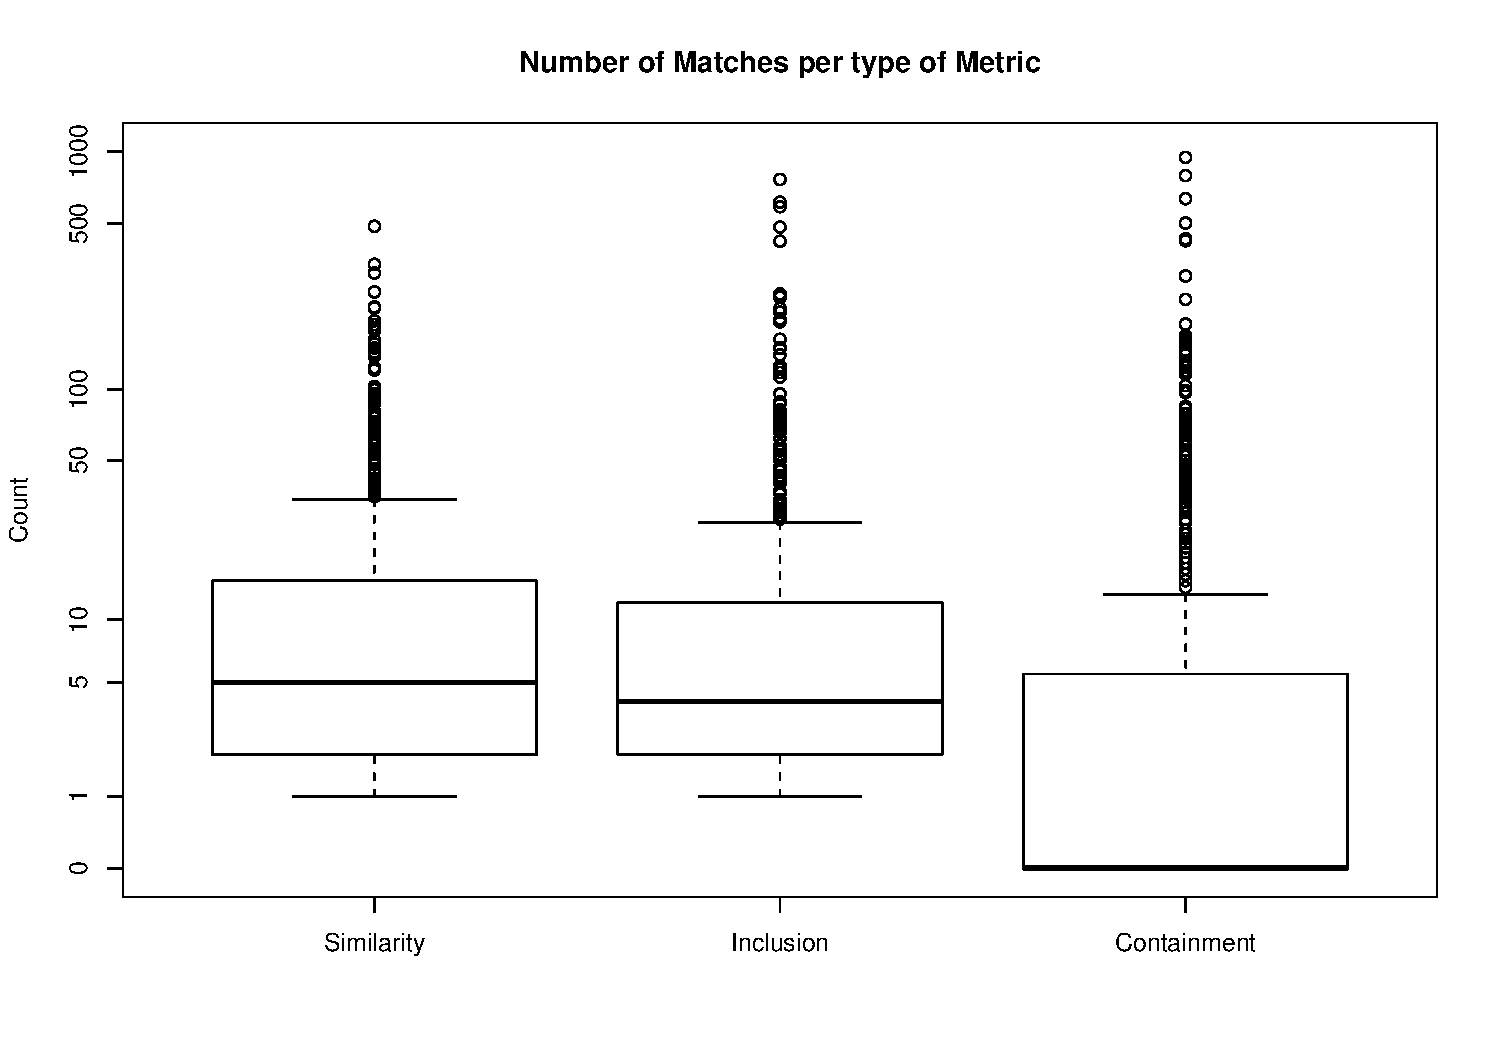
\includegraphics[width=\columnwidth]{plots/boxplotPerfectMatches.pdf}  
\vspace{-7mm}
  \caption{Number of top-matches found in the binary-to-binary
    experiment. The different metrics had a median of 5 or 6 matches,
    but they had long tails, suggesting a lot of duplication of some
    jars in the sample. }
  \label{fig:topMatchesSource}
\end{figure}


\subsubsection{Binary-to-source matching results}
%-- Results, binary to source.

For each of the 1,000 archives in the sample set we computed its similarity
with every source archive in the repository.  While we satisfied ourselves
that our extractors worked as expected, the exploration of the Maven
repository yielded some surprising results:

We classify the result of a search into three three categories:

    \begin{enumerate}
    \item The correct match was among those with the top matching Similarity
	index (966 cases out of 1,000).
    \item The correct match had a lower Similarity index than some
	other archives (30 cases).
    \item The algorithm failed to suggest any matches (4 cases).
    \end{enumerate}

In 966 of the 1,000 archives in the sample set, the correct match was among
those with the top Similarity Index.  The median Similarity Index of a
binary archive and its corresponding source archive was 1.0.  However,
there were several cases where the correct source match had a surprisingly
low Similarity Index, with the lowest in our sample set being 0.0290.  Low
Similarity indexes typically indicate that dependent archives have been
added within the binary version of the archive; for example, the source
Java files in \mytt{rampart-integration-1.5.1.jar} have 12 signatures, yet
its binary version contains 231 signatures (those of classes it uses as
dependencies, and that are embedded in the jar to avoid having to
independently install them in the running environment).  The distribution
of the top number of source packages matching the top Inclusion Index is
shown in figure~\ref{fig:topMatchesSource}.  

If there are multiple top matches for a given archive --- that is, if there
are multiple archives with the same maximal Inclusion index when compared
to the candidate archive --- then a more detailed examination of them must
be performed.  Typically, this means that there are multiple versions of
the archive that have an identical interface; that is, the implementation
may have evolved between versions but the interface stayed consistent.  In
our sample set, we found that the minimum number of top matches was 1, and
the median was 4.  However, there were a few cases where the number of top
matches was large; the most extreme case was
\mytt{maven-interceptor-1.380.jar} for which we found 158 different
versions from 1.237 to 2.0.1.  

We were not able to match any source in 4 cases.  These were all small
archives consisting of between one and three classes each, and in each of
these cases the compiler, or other bytecode manipulators had added various
fields and methods that were not actually in the source code.  While we are
aware of this phenomenon, our extractor does not explicitly handle such
fields and methods.


And finally, we noted that in 30 cases, the top match was not the correct
match.  Manual inspection suggests that in these cases the binary jars had
embedded within them external dependencies from other archives whose
numbers exceeded those of the source itself.  For example,
\mytt{org.apache.felix. http.bundle-2.0.2-sources.jar} contains only one
Java file, yet its binary equivalent \mytt{org.apache.felix.http.bundle.2.0.2.jar}
contains 295 signatures (in 442 .class files); other binary
packages with a higher Inclusion Index were \mytt{servlet-api-2.5}
(contributing 145 signatures) and \mytt{jetty-6.1.*}, contributing 13
classes.  This brings up an interesting philosophical question: What is the
source of a given binary?  Is it the source it was created from, or the
dependencies it contains?  Certainly all of them, and our method shows
this. 

Of these 30 cases, 10 source files have a Containment Index of 1.0 (their
binary jar perfectly contains all the signatures in the source file). In
other words, while the expected source was not the top match for the
Similarity Index, it was for the Containment one.

%  \migod{Below are Daniel's original comments, which I need some help
% understanding.}

% Not top match: 30. In other words, for 30 jars the source file
%   in the same directory was not the best match. We analyze few of
%   these files, and discovered that the main reason they did not match is
%   because the binary jars are also embedding dependencies from other
%   packages, and these dependencies are larger than the source itself. For
%   example, \mytt{org.apache.felix.http.bundle-2.0.2-sources.jar} contains
%   only 1 Java file, yet its binary equivalent:
%   \mytt{org.apache.felix.http.bundle-2.0.2.jar} contains 295 signatures (in
%   442 .class files). The Bertillonage metrics show that it contains 41
%   files from \mytt{servlet-api-2.5}, and 145 and from jetty-6.1.*., 13
%   classes from \mytt{org.apache.felix.http.whiteboard-2.0.*}.
  
%   This really brings something interesting: what is the source of the
%   binary? Is it the one that created it, or the dependencies it contains?
%   Certainly both, and the Bertillonage metrics show it.

%   Of there 30 cases, 10 source files have a Containment metric of 1.0
%   (they binary jar perfectly contains all the signatures in the source
%   file).

%-- \begin{itemize}
%-- \item Top match: 966. For these, the expected source was listed as the top
%--     match. The values are: Min.  :0.0290 , Median 1.00, Max, 1.000. In
%--     fact, only 10\% (98) had a Jaccard less than 1. Those with low Jaccard
%--     reflected packages that included dependencies into the binary (e.g.
%--     \mytt{rampart-integration-1.5.1.jar} has 12 signatures, yet it binary
%--     has 231 ones). The distribution of the top number of source packages
%--     matching the top Jaccard is shown in figure~\ref{fig:topMatchesSource}.
%--     At is can be seen, the median number of top matches is very small:
%--     min1, max 158, median 4, but in few cases.  The largest set of matches
%--     (158) correspond to \mytt{maven-interceptor-1.380.jar} to 158 different
%--     versions of it, from 1.237 to 2.0.1.
%--  
%-- \item We were not able to match any source in 4 cases. The reasons are:
%--     very small packages (1,1,2, and 3 classes) for which the compiler adds
%--     fields and methods to the class that are not in the source. These are
%--     not handled by our parser.

%/maven/org/ow2/jasmine/monitoring/jasmine-monitoring-integration-tests-modules-events/1.2.5/jasmine-monitoring-integration-tests-modules-events-1.2.5.jar
%/maven/org/ow2/jasmine/monitoring/jasmine-monitoring-integration-tests-modules-events/1.2.5/jasmine-monitoring-integration-tests-modules-events-1.2.5-sources.jar 
%
%This one has some fields in the class that are not in the source:
%
%f;0;  private InstanceManager __IM;
%f;0;  private boolean __Flogger;
%...
%f;0;  private boolean __Mstart;
%m;0;  Logger __getlogger()
%m;0;  void __setlogger(Logger)
%-- \item Not top match: 30. In other words, for 30 jars the source file
%--   in the same directory was not the best match. We analyze few of
%--   these files, and discovered that the main reason they did not match is
%--   because the binary jars are also embedding dependencies from other
%--   packages, and these dependencies are larger than the source itself. For
%--   example, \mytt{org.apache.felix.http.bundle-2.0.2-sources.jar} contains
%--   only 1 java file, yet its binary equivalent:
%--   \mytt{org.apache.felix.http.bundle-2.0.2.jar} contains 295 signatures (in
%--   442 .class files). The Bertillonage metrics show that it contains 41
%--   files from \mytt{servlet-api-2.5},  and 145 and from jetty-6.1.*., 13
%--   classes from \mytt{org.apache.felix.http.whiteboard-2.0.*}.
%--   
%--   This really brings something interesting: what is the source of the
%--   binary? Is it the one that created it, or the dependencies it contains?
%--   Certainly both, and the Bertillonage metrics show it.
%-- 
%--   Of there 30 cases, 10 source files have a Containment metric of 1.0
%--   (they binary jar perfectly contains all the signatures in the source
%--   file).
%-- 
%-- \end{itemize}


\begin{figure}[h]
  \centering
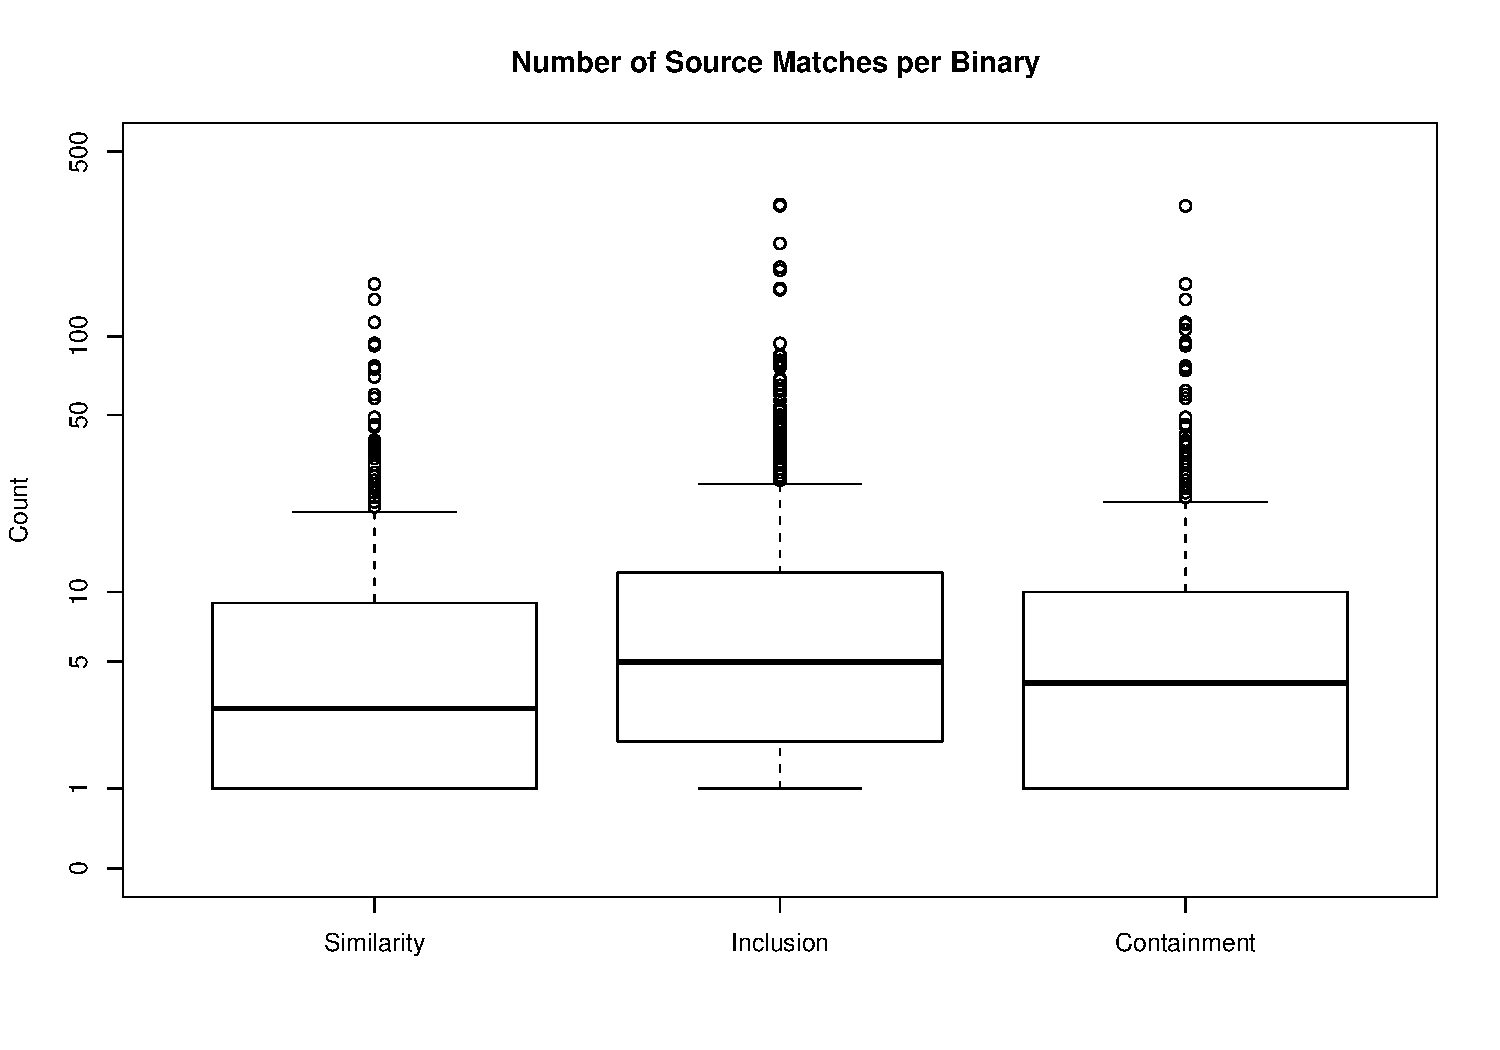
\includegraphics[width=\columnwidth]{plots/boxplotAllMatches.pdf}  
\vspace{-7mm}
  \caption{Matching sources: Number of matches for each metric}
  \label{fig:matchesMetric}
\end{figure}


\subsubsection{Summary of Exploration and Tool Evaluation}

In summary, to evaluate our tools and to explore the problem space
of the Maven repository, we applied our techniques to 1,000 binary
archives, randomly chosen from Maven but with the constraint that the
sources also be present in Maven.  In 96.6\% of the cases (margin of
error of 4\% with a confidence level of 99\%) we were able to match
the binary of a source using (one of) the top Similarity Index
match(es). In 3\% of the cases the best match was not the correct
source (but the correct one had a slightly lower similarity index and
was part of the set of candidates). In 0.4\% of the cases, we could not match
the source at all.
% ; however, in
% each of these cases the archives were very small so manual matching
% would be quick.

Overall, our metrics-based approach appears to be effective for
significantly narrowing the search space when looking for matches for
another binary (the median number of top matches was 5). In the few
occasions it failed to find a match (0.4\%), the archives were very small
and the compiled classes were built using features (e.g., direct bytecode
manipulation) that our parser was not able to process.

When matching binary packages to their corresponding source, we identified
several commonalities. In many cases, the binary and the source were a
1-to-1 match, but in many other cases, the binary was a superset of the
source archive (it contained the dependencies that it required to
function). In this case, the containment metric is useful: it shows us that
the binary package contains the source packages.  We found it interesting
that in few cases, the best-match was not the corresponding source, but one
of its dependencies.  In other cases, the best match was a subset of the
binary archive. This is common when a source archive is split into several
binary packages, or when there exists a large number of test cases that are
not included in the binary. In these cases the inclusion metric is the best
to use.

% \begin{itemize}
% \item Overall, the Jaccard metric is a very effective method to narrow
%   the search space when looking for the source code of a binary. The
%   median number matches one would need to analyze was 5.
% \item In many cases a binary package would contain classes not present
%   in the sources. These are typically dependencies. Sometimes these
%   dependencies might be more numerous than the number of Java files in
%   its source. The Jaccard and Inclusion metric can be very useful to
%   identify such packages.
% \item Some binary packages are ``super containers'' that are composed
%   of numerous binaries that come from different products.
% \item For very few packages, the signatures do not change over a long
%   period of time.
% \end{itemize}




%%% Local Variables: 
%%% mode: latex
%%% TeX-master: "000_main"
%%% End: 


\section{Evaluation}\label{sec:evaluation}

\label{sec:method}

To validate any provenance technique we need a sample of artifacts from
outside our corpus, and we need ``ground truth'' about these artifacts.  We
can then apply our technique to determine provenance information about each
of the sampled artifacts and compare the answers returned with the ground
truth.  However, we have a confounding variable.  We do not possess a
perfect corpus.  Should our technique fail, do we blame our method for
indexing the artifacts, or do we blame imperfections in the corpus?

To control for this variable, we assume that byte-oriented fingerprinting
techniques are valid.  By applying byte-oriented fingerprinting techniques
alongside our Bertillonage technique, we introduce a baseline against which
our new technique can be objectively measured.  With the validity of our
technique firmly established, we can then use our corpus and our sampled
artifacts to further explore the following research questions:



\vspace{0.7em}

% RQ1 = How well does bin2bin work?
\textbf{RQ1}: \textbf{\rqOne}

%Should we use binary fingerprint indices,
%where only exact byte-for-byte matches are possible?  Or should we use
%Bertillonage indices, such as anchored signature matching, to expand our
%range of possible matches?

\vspace{0.7em}

% RQ2 = How well does bin2src work?
\textbf{RQ2}: \textbf{\rqTwo}

% RQ2 = Is Maven a good corpus?
%Or can a corpus such as the Maven2 Central Repository, with its incompleteness, redundancy, and disorganization,
%still be useful?
%Is there a set of characteristics a corpus should possess to be considered ``good enough'' for provenance analysis?

\vspace{0.7em}

% RQ3 = Are jar names reliable?
\textbf{RQ3}: \textbf{\rqThree}


% RQ3 = Can we find the source?
%This is the hard problem of provenance, as it relates to compiled computer programs:
%given a binary, can we find its source?   Byte-for-byte fingerprint approaches fail here, of course,
%since the original (the answer) is a transformation of the subject (the question).
%Our Bertillonage technique is designed as an exploratory stab
%at this problem, and as such, what do we learn?



%Since provenance is important to software
%developers, name and release is often encoded directly into an artifact's file name
%(e.g., oro-2.0.7.jar).  Nonetheless developers may omit the release numbering, or
%they may mistype it.  Also, in some cases an artifact internally encompasses additional 
%artifacts, rendering the file name inadequete for communicating the versions of the encompassed
%releases.  RQ3 considers the artifact's file name as a baseline technique for
%determining provenance against which RQ2 and RQ1 can be compared.  How
%often is the filename incorrect, and how often is the filename simply inadequete?
%Is the additional expense of building the index and executing the queries for
%anchored signature matching worth the trouble?


\subsection{Setting}

%\abram{ explain setting  }

\subsubsection{Building A Corpus}

We mirrored the Maven2 central repository (from July 25th to July 30, 2011) using the
following command:

\hspace{2em} \quad{\mytt{rsync -v -t -l -r mirrors.ibiblio.org::maven2 .}}
\vspace{0.3em}

We used the \mytt{ibiblio.org} mirror because \mytt{repo1.maven.org}
does not allow unknown parties direct connections via \mytt{rsync};
\mytt{repo1.maven.org} also bans HTTP crawlers.
Our download from \mytt{ibiblio.org} averaged 350KB/second.
Since we retained our initial 150GB mirror from a year earlier
the \mytt{rsync} command needed to only download the remaining 125GB
of artifacts, requiring 4 days to download.  We re-ran the \mytt{rsync} command
on the final day of downloading (June 30th)
to ensure that our version was more or less identical to the ibiblio
mirror at that time.
Thus we obtained over 275 GB of jars, zips, tarballs, and other files.
Maven contained 360,000\footnote{Values are rounded to nearest 10,000.}   
% non-rounded:     359,421
different archives (\mytt{.tar}, \mytt{.zip}, \mytt{.tar}, \mytt{.war},
\mytt{.tgz}, \mytt{.ear}, and \mytt{.jar}). Many of them contained other
archives within them.  When uncompressed, they resulted in 130,000
% non-rounded:    130,738
source archives (a source archive contains at least one Java file), but
only 110,000 
% non-rounded:    106,723
were unique.  It contained 650,000                                    
% non-rounded:    647,763
binary archives (each contained at least one class file), but only 140,000
% non-rounded:    144,049
were unique.  These archives contained 7,140,000
% non-rounded:  7,139,261
Java files (1,650,000                                                 
% non-rounded:  1,648,594
distinct), and these generated 920,000 unique signatures.                 
% non-rounded:    921,690

We processed  19,780,000                                              
% non-rounded: 19,775,475
class files (2,430,000  distinct)\footnote{We only count outter classes.
Class files containing a \mytt{\$} (dollar-sign) character in their name are assumed to be inner classes,
and are not included in these tallies.  For example, only 3 of the class files listed earlier in Table~\ref{tab:asym} would count:
\mytt{A.class}, \mytt{B.class}, and \mytt{C.class}.  These do not contain
\mytt{\$} in their names, whereas the other 4 classes do.}
% non-rounded:  2,431,413
which generated  1,510,000                                             
% non-rounded:  1,509,761
distinct signatures.  We observed there are 590,000 (or 39\%) fewer
distinct signatures among our source files compared to our class files.
This is despite the observation that a typical source archive often
contains more signatures than its corresponding binary archive, since the
source archive is more likely to contain unit tests.  This discrepancy
suggests Maven contains many binary archives for which there is no source
code, a fact we confirmed previously in section~\ref{sec:mavenExplore}.

We used the Canada Western Research Grid~\cite{WCRG} to extract these signatures. The
extraction took approximately 8 hours, which was equivalent to 325 hours of a
single CPU. Once the signatures were extracted, a PostgreSQL database was
created from the results; the database was 11GB in size (including indexes).
Bulk loading the compressed data (pre-sorted) directly from disk into two tables
required 30 minutes on an Intel Core i3 laptop with a 7200 RPM hard-drive.
Creating five single-column indexes required 90 minutes.
A final 3 hours was spent pre-computing distinct signature tallies
for each jar file.  In total 5 hours were spent creating the database from the
extracted data.

Initial bertillonage queries of our database ran very slowly, taking several minutes
per jar file analyzed.
Our \mytt{WHERE} clauses contain long chains of \mytt{OR} conditions, e.g., a typical
SQL query from our tool looks like
\mytt{WHERE sig=\emph{class1} OR sig=\emph{class2} OR sig=\emph{class3}...}, and may include several thousand
of these \mytt{OR} conditions,
one for each class in the jar file.
We realized that PostgreSQL's query optimizer, when planning these huge \mytt{WHERE} clauses,
was erroneously assuming full-table scans would run faster than index scans.
We tuned PostgreSQL's query optimizer to avoid full-table-scans whenever
possible by setting \mytt{enable\_seqscan = off} in the configuration file.
This resulted in most queries taking less than one second, with the slowest queries
requiring at most 20 seconds.  Section~\ref{perf} contains additional concrete
performance details about our implementation.



\subsubsection{Experimental Subjects:  945 Jar Files From Debian 6.0}

To obtain a sample of artifacts outside our corpus we looked at the Debian
GNU/Linux distribution.  Many Java libraries are compiled into discrete,
installable packages in this large operating system.  The packages, called
\emph{Debs}, include name, version, and dependency information that is
recorded by Debian maintainers.  These maintainers often possess
familiarity and expertise related to the packages they oversee, thus we are
confident the provenance information recorded by these experts is of high
quality, and can be considered reasonably close to ground truth.  The Deb
format can be used to package any type of installable application, not just
Java applications, but for our purposes we looked only at packages
containing Java libraries.  We chose the most recent stable release, Debian
6.0 ``Squeeze'', released on February 6th, 2011, from which to collect
packaged Java artifacts.

Debian 6.0 contains over 1,750 Java jar files.  However, in some cases we
noticed the provenance information recorded by the Debian package
maintainers was nuanced and complex, and required time and effort to
properly understand.  For example, one particular Debian package,
\mytt{libgdata-java\_1.30.0}, was specified as version 1.30.0, and yet
the jars inside this package were marked with a variety of version numbers:

\begin{itemize}

\item \mytt{libgdata-java\_1.30.0-1\_all.deb/gdata-core-1.0.jar}
\item \mytt{libgdata-java\_1.30.0-1\_all.deb/gdata-docs-2.0.jar}
\item \mytt{libgdata-java\_1.30.0-1\_all.deb/gdata-photos-1.0.jar}
\item \mytt{libgdata-java\_1.30.0-1\_all.deb/gdata-youtube-2.0.jar}
\item etc...

\end{itemize}

None of these jars included the version `1.30.0' within their own names.
To make our analysis easier, we decided to filter out all jars that did not
include the same version number in their name as that of their containing
package.  In this way we reduced our sample from 1,750 jars down to 945.
We believe this filtering further improves the ground
truth of our sample, since the version is specified in two places for each
jar.  In a way, each jar possesses two `votes' regarding its encoded
version information.

We are not attempting to validate byte-oriented fingerprint techniques,
such as SHA1.  We assume byte-oriented fingerprint techniques work, and we
use them as a measuring stick from which to compare our signature based
Bertillonage technique.  We assume fingerprint approaches achieve 100\%
precision, and that false positives are impossible.\footnote{The chance of
a birthday collision from SHA1 in our data set is less than $10^{-18}$.}
For fingerprints of archive files, any match is considered equivalent to
ground truth, even if the matched name is different, since they are
byte-for-byte identical.  Similarily, for fingerprints of archive contents,
any match that scores 1.000 similarity is considered equivalent to ground
truth.  Fingerprint matches of archive contents scoring 0.999 similarity or
less are \emph{not} considered ground truth, and if they represent the best
match, we consider these as experimental results for validation, rather
than ground truth for measuring against.


\subsubsection{Replicating An Industrial Case Study}

In a related research project~\cite{Davies11} we performed a license
and security audit of a real world e-commerce application.  The audits had
to be performed against both the binary and source code forms of these
included libraries.  Before we could conduct the audits, we needed to
determine the provenance of all included libraries.  In this study we
replicate the provenance phase using 81 jars from the other project's
replication package.\footnote{http://juliusdavies.ca/2011/icse/src/}

Accurate and precise provenance information forms an important foundation
for many types of higher-level analyses.  Such analyses include, among
others, license audits, security vulnerability scans, and patch-level
assessments (as required by the PCI DSS security standard).  A license
audit of software dependencies must reflect the reality that software
licenses sometimes evolve (change between releases).  Similarily, known
security holes in libraries will affect specific releases or version
ranges.  The PCI DSS requirement \#6, ``All critical systems must have the
most recently released, appropriate software patches,'' cannot be satisfied
without knowledge of the existing patch versions.  In this vein we believed
that conducting a license audit and a security audit would provide real
value to the developers of the e-commerce application, while also providing
us with a chance to test our Bertillonage approach in the field.



%We applied our technique in two different modes,  binary-to-binary, and source-to-binary.






% RQ1 = What kind of index to use?

% RQ2 = Is Maven good enough?

% RQ3 = Can we find the sources?

%For RQ1, for each of the 81 e-commerce jars, we computed their
%similarity index against every binary archive in the corpus,
%and selected the set of matches with the highest similarity
%as the binary archive match.

%For RQ2, the same procedure is performed as in RQ1, but instead
%the similarity index is computed against every source archive
%in the corpus.
%For RQ1 and RQ2 we classified a match into one of three categories:

\subsubsection{Measuring Results}

We define one byte-oriented index (``Fingerprint Index"), and one
Bertillonage index (``Anchored Class Signature Index").  Using the indices,
we define four matching techniques (two per index).  Here are the four
matching techniques, followed by a shorthand tag we use later to refer to
them.

\begin{description}
\item \textbf{Fingerprint Index, Identical Archive} (sha1-of-jar)

Our fingerprint index stores SHA1 fingerprints of all archive files, as
well as all source and class files.  Therefore, an easy way to query the
corpus is to simply take the SHA1 fingerprint of the subject archive and
see if anything matches.   A match found in this way represents a
byte-for-byte identical copy of the subject archive.  We also use this
index to filter out duplicate results reported by the other matching
techniques.

\vspace{0.7em}
\item \textbf{Fingerprint Index, Identical Contents} (sha1-of-classes)

This matching technique scans a subject archive to generate a series of
SHA1 fingerprints, one per class scanned.  We then query the corpus using
the same \emph{similarity}, \emph{inclusion}, and \emph{containment}
metrics described earlier.  But instead of comparing sets of anchored class
signatures, we compare sets of bytecode.  Some pre-processing is required
to properly account for inner-classes, since we want a change to the
inner-class's bytecode to effect the outer class's fingerprint, even in
cases where the outer class did not change (rare, but we observed some
instances).

\vspace{0.7em}
\item \textbf{Anchored Class Signature Index, Binary-To-Binary} (bin2bin)

Here we use our Bertillonage technique to find matches as described in
section~\ref{sec:finding}.  For each jar file in our sample we extract the
signatures from the bytecode, and we build a query from these signatures.
The query is configured to only examine matching \emph{binary} signatures in the corpus.


\vspace{0.7em}
\item \textbf{Anchored Class Signature Index, Binary-To-Source} (bin2src)

Again we use our Bertillonage technique to find matches as described in
section~\ref{sec:finding}.  We examine the bytecode in each jar file, but
in this case the query is configured to examine matching \emph{source} signatures in
the corpus.  


\end{description}

\vspace{0.7em}

\noindent We classify matches into one of three quality levels: High
Quality (HQ), Low Quality (LQ), and No Match.  We further divide each
quality level into subcategories that communicate our criteria for
evaluating match quality.  These subcategories also allow us to report some
cross-tabulated results, so we can directly compare results between the
four matching techniques.


\begin{enumerate}
\item \textbf{High Quality (HQ):} 
    To be considered a high quality match, the top-ranked set of matches
    (those tied for best similarity score) must contain one candidate that
    satisfies one of the following four conditions:

\begin{itemize}

\vspace{0.7em}
\item \textbf{\emph{HQ1.} Identical archive:}
    The candidate is a byte-for-byte identical match, regardless of name or
    version information encoded in the candidate's name.

\vspace{0.7em}
\item \textbf{\emph{HQ2.} Identical contents:}
    The contents of the candidate (class files) all match byte-for-byte
    with the contents of the subject.  There are no unmatched contents in
    either the candidate or the subject.  These matches are considered
    successful regardless of name or version information encoded in the
    candidate's name.

\vspace{0.7em}
\item \textbf{\emph{HQ3.} Expected match:}
    The candidate's name and version information is identical to the
    expected name and version information.

\vspace{0.7em}
\item \textbf{\emph{HQ4.} Version off by final digit:}
    The candidate's name is identical, and the version information is only
    different in its final character, e.g., a match of
    \mytt{ezmorph-1.0.4.jar} against ground truth of
    \mytt{ezmorph-1.0.6.jar} is considered a high quality match.

\end{itemize}

\vspace{0.7em}
\item \textbf{Low Quality (LQ):}
      Any match that is not classified as high quality is classified as low
      quality.  We further subdivide low quality matches into two types:

\begin{itemize}

\vspace{0.7em}
\item \textbf{\emph{LQ1.} Version off by many digits:}
    The candidate's name is identical but the version information is
    different, and this difference is not just in the final digit, e.g.,  a
    match of \mytt{serp-1.13.1.jar} against ground truth of
    \mytt{serp-1.14.1.jar} is considered a low quality match.  Also
    matches where we knew the candidate's name was an older name for the
    library are also classified in this category, e.g.
    \mytt{xml-apis-2.0.2-sources.jar} was classified as a LQ1 match
    against \mytt{crimson-1.1.3.jar} rather than a LQ2 match because we
    happened to know the library had changed its name from `crimson' to
    `xml-apis.'

\vspace{0.7em}
\item \textbf{\emph{LQ2.} Not useful:}
    The candidate's name and version information did not provide
    information useful for provenance analysis.  Due to the \emph{anchored}
    nature of our signatures, these are not false positives.  Remnants of
    past cloning, branching, or merging often show up in many of our
    queries, but these fragments usually sit near the bottom of the
    returned results, with low \emph{similarity} scores.  However, when a
    hole in our corpus precludes the correct match, these fragments can
    achieve the highest score.  We say these results are not useful for
    provenance analysis.  Users may nonetheless find these results useful
    for other purposes, such as evolution, cloning, or descendant analyses.




\end{itemize}

\vspace{0.7em}
\item \textbf{No Match}
      While not technically a type of match, this is an important category.
      In all experimental and case-study results a portion of the sampled
      artifacts result in no matches at all.

\end{enumerate}


%%% Local Variables: 
%%% mode: latex
%%% TeX-master: "000_main"
%%% End: 

\subsection{Results I:  The Experiment}

\label{sec:results}

This section reports results of analyzing 945 jar libraries extracted from
Debian 6.0 Squeeze to answer the research questions formulated 
%-- in Section~\ref{sec:method}.  
at the beginning of this section.
By treating version and name information encoded
in the 945 Debian jar files as a good approximation of ground truth, we can
compare our signature-based Bertillonage technique against a baseline
technique.

Our techniques consider only the top match according to our
\emph{similarity} metric, as described in Section~\ref{sec:sim}.  Often the
top similarity score is shared by several artifacts in our corpus.  As
evidenced by the results, 2-way, 3-way, and 4-way ties for best similarity are the
norm, rather than the exception.  However, to understand what we mean by a
\emph{tie}, we must mention briefly what we consider \emph{a single
artifact}.  Our earlier exploration of the Maven2 corpus (see
Section~\ref{sec:mavenExplore}) shows surprising redundancy and duplication
of archives within the repository.  Users are likely not interested in knowing all two hundred
path locations of an identical artifact.  We filter out these duplications
and instead report only ties that either have a different SHA1 binary
fingerprint than other matches in the tie, or a different name.  

In some cases choosing a top match based on the inclusion metric rather
than similarity performs better.  To keep our experiment simple, we
consider these to be wrong matches.  We anticipate future researchers
will improve on our results by tuning the match criteria to factor in
both similarity and inclusion scores when selecting the \emph{top} match,
perhaps at a cost of larger \emph{ties}.


\subsubsection{The Baseline:  Binary Fingerprint Matches}

\begin{table}[h]
  \centering
\begin{tabular}[htbp]{l|r|lll|rrr}
  sha1-of-class/Debian-945   &              & \multicolumn{3}{c|}{\textbf{Similarity}}  & \multicolumn{3}{c}{\textbf{\# of Ties}} \\
  \textbf{Type of Match}     & Count        & Min   & Mdn    & Max   & Min  & Mdn  & Max  \\
\hline
%& & & & & & & \\
  \emph{HQ1.} Identical archive          &   2          & 1.0   & 1.0    & 1.0   & 1    & 1    &  1   \\
  \emph{HQ2.} Identical contents         & 201          & 1.0   & 1.0    & 1.0   & 1    & 1    & 35   \\
  \emph{HQ3.} Expected match             & 131          & 0.014 & 0.680  & 0.997 & 1    & 1    & 13   \\
  \emph{HQ4.} Version off by final digit &  49          & 0.033 & 0.500  & 0.977 & 1    & 1    &  4   \\
  \emph{\textbf{High Quality Matches}}   & \textbf{383} &       &        &       &      &      &      \\
& & & & & & & \\
  \emph{LQ1.} Version off by many digits &  85          & 0.001 & 0.116  & 0.964 & 1    & 1    & 25   \\
  \emph{LQ2.} Not useful                 &  22          & 0.003 & 0.025  & 0.206 & 1    & 1    & 18   \\
  \emph{\textbf{Low Quality Matches}}    & \textbf{107} &       &        &       &      &      &      \\
& & & & & & & \\
  \emph{\textbf{No Matches}}             & \textbf{455} &       &        &       &      &      &     \\
%& & & & & & & \\
\hline
  \textbf{Total Matches:} \hspace{3em} \textbf{(52\%)} & \textbf{490}   & \multicolumn{3}{c|}{\textbf{Average: 0.685}}  & \multicolumn{3}{c}{\textbf{Average: 2.4}} \\
\end{tabular}
  \caption{The baseline results:  matches are based on binary SHA1 fingerprints of the 945 Debian jars.}
  \label{tab:debianSha1OfClass}
\end{table}


\begin{table}[h]
  \centering
\begin{tabular}[htbp]{r|r|r}
\textbf{Tie \#}  & \textbf{Similarity} & \multicolumn{1}{c}{\textbf{Version}} \\
\hline
1.        & 1.0 &          plexus-component-annotations-1.0-alpha-1.jar  \\
2. - 17.  & 1.0 &                            \multicolumn{1}{c}{\emph{alpha-2 - alpha-17}}  \\
18.       & 1.0 &           plexus-component-annotations-1.0-beta-1.jar  \\
19. - 27. & 1.0 &                   \multicolumn{1}{c}{\emph{1.0-beta-2 - 1.0-beta-3.0.6}}  \\
\textbf{28.}       & \textbf{1.0} &       \textbf{plexus-component-annotations-1.0-beta-3.0.7.jar}  \\
29. - 34. & 1.0 &                                 \multicolumn{1}{c}{\emph{1.0 - 1.2.1.3}}  \\
35.       & 1.0 &              plexus-component-annotations-1.2.1.4.jar  \\
\end{tabular}
  \caption{
    We found 35 top matches with
    \mytt{plexus-component-annotations-1.0-beta- 3.0.7.jar} when using
    binary fingerprint matches.  Notice how candidate \#28 contains the
    same name as the subject archive, hence this match could be classified
    as `HQ3. Expected Match.' However, we consider all 1.0 similarity
    matches of SHA1 fingerprints as ground truth, hence this match's
    classification as `HQ2. Identical Contents.' A relatively small jar,
    \mytt{plexus-component-annotations-1.0-beta-3.0.7.jar} contains only 3
    classes.  
}
  \label{tab:sha1-of-class-35-matches}
\end{table}

Table \ref{tab:debianSha1OfClass} shows the results of our baseline
technique, a straightforward SHA1 index of jar files and class files.
Slighly over half the Debian sample, 490 jars out of 945 (52\%), contained
one or more class files that were identical to a class file in the Maven
corpus.  Each match returned an average of 2.4 candidates that tied for top
similarity.  The match with the most ties among our baseline results is
shown in Table \ref{tab:sha1-of-class-35-matches}.  The average score of
the 490 best similarity scores was 0.685.

Only 2 out of the 945 jar files proved to be identical complete archive
copies from the Maven corpus (row \emph{HQ1}).  We suspect the main reason
for such a low match percentage (less than 0.5\%) in this category may be
Debian's policy of recompiling all jar files from original sources.  Jar
files record timestamps of contained files, and Java class files tend to
have timestamps set to the moment they were compiled.  This alone will
cause Debian jar files to differ, at least in a few bytes, from their Maven
counterparts.  A further 201 out of the 945 jar files matched with
identical contents (\emph{HQ2}).  These 201 matches, while externally
different, were internally identical with respect to contained class files.
Of course the 2 identical jar files also matched according to contents.

A remaining 287 jar files had partial matches, with similarity scores less
than 1.0.  Of these, 180 matches, when evaluated against our ground truth,
scored as high quality matches (\emph{HQ3} to \emph{HQ4}), and 107 matches
scored as low quality matches (\emph{LQ1} to \emph{LQ2}).  Finally, for 455
jars, there were no matches at all using the binary fingerprint technique.


\subsubsection{The First Test: Binary-to-Binary Anchored Signature}

\begin{table}[h]
  \centering
\begin{tabular}[htbp]{l|r|lll|rrr}
  bin2bin/Debian-945         &              & \multicolumn{3}{c|}{\textbf{Similarity}}  & \multicolumn{3}{c}{\textbf{\# of Ties}} \\
  \textbf{Type of Match}     & Count        & Min   & Mdn    & Max   & Min  & Mdn  & Max  \\
  \hline
%& & & & & & & \\
  \emph{HQ1.} Exact (sha1 of jar)        &   2          & 1.0   & 1.0    & 1.0   & 1    & 1.5  &  2   \\
  \emph{HQ2.} Exact (sha1 of *.class)    & 201          & 1.0   & 1.0    & 1.0   & 1    & 3    & 86   \\
  \emph{HQ3.} Expected match             & 442          & 0.046 & 1.0    & 1.0   & 1    & 2    & 30   \\
  \emph{HQ4.} Version off by final digit &  65          & 0.038 & 0.889  & 1.0   & 1    & 1    & 23   \\
  \emph{\textbf{High Quality Matches}}   & \textbf{710} &       &        &       &      &      &      \\
& & & & & & & \\
  \emph{LQ1.} Version off by many digits &  67          & 0.014 & 0.414  & 1.0   & 1    & 1    & 14   \\
  \emph{LQ2.} Not useful                 &  16          & 0.002 & 0.027  & 0.807 & 1    & 1    &  4   \\
  \emph{\textbf{Low Quality Matches}}    & \textbf{83}  &       &        &       &      &      &      \\
& & & & & & & \\
  \emph{\textbf{No Matches}}             & \textbf{152} &       &        &       &      &      &     \\
%& & & & & & & \\
  \hline
  \textbf{Total Matches:} \hspace{3em}    \textbf{(84\%)} &  \textbf{793}   & \multicolumn{3}{c|}{\textbf{Average: 0.890}}  & \multicolumn{3}{c}{\textbf{Average: 3.5}} \\
\end{tabular}
  \caption{bin2bin Bertillonage --- our signature-based approach applied to
    945 Debian jars.} 
  \label{tab:debianBin2Bin}
\end{table}


\begin{table}[h]
  \centering
\begin{tabular}[htbp]{r|r|l|l}
\textbf{Match \#}  & \textbf{Similarity} & \textbf{Inclusion} & \multicolumn{1}{c}{\textbf{Match}} \\
\hline
1.        & 0.046 & 1.0   &         javahelp-2.0.05.jar \\
2.        & 0.041 & 0.889 &         javahelp-2.0.02.jar \\
\end{tabular}
  \caption{
    In this anchored signature example the top match for
    \mytt{jsearch-indexer-2.0.05.ds1.jar} had a low similarity score. Only
    9 of \mytt{javahelp-2.0.05.jar}'s 195 signatures matched.  We
    classified this as HQ3. ``Expected match,'' since it resided inside a
    Debian package named \mytt{javahelp2\_2.0.05.ds1-4\_all.deb}, and so
    name and version did match as expected.  Because this match also
    possessed a 1.0 inclusion score, we suspect the Debian maintainers are
    splitting a large jar (which exists in Maven) into several smaller jars
    (which do not).  }
  \label{tab:046similarity}
\end{table}

Table \ref{tab:debianBin2Bin} shows the results of our first Bertillonage
test:  binary-to-binary anchored signature matching.  In the Debian sample,
we found that 793 jars out of 945 (84\%) contained one or more class files
with an identical anchored signature as a class file in the Maven corpus.
Each match returned an average of 3.5 candidates that tied for top
similarity.  The average score of the 793 best similarity scores was
0.890.  The highest quality match with the lowest similarity score (0.046)
is shown in table \ref{tab:046similarity}.

We found that 710 matches, when evaluated against our ground truth, scored
as high quality matches (\emph{HQ1} to \emph{HQ4}), and 83 matches scored
as low quality matches (\emph{LQ1} to \emph{LQ2}).  Finally, for 152 jars,
there were no matches at all using anchored signature binary-to-binary
matches.  In general our Bertillonage approach outperformed the baseline,
with nearly twice as many high-quality matches (710 vs.\ 383), fewer
low-quality matches (83 vs.\ 107), and far fewer non-matches (152 vs.\ 455).

As expected, all binary-identical matches also scored 1.0 for
signature-similarity, as shown in the two crosstab rows (\emph{HQ1} to
\emph{HQ2}).  Any non-perfect score in these rows would signify a critical
bug in our tool, since a binary-identical class-file should also possess an
identical signature.  One interesting difference, however, is the increase
in ties in the crosstab rows.  The anchored signature approach exhibited a
higher median (3 vs.\ 1), a higher maximum (86 vs.\ 35), and the overall
average tie rate was also higer (3.5 vs.\ 2.4).  These differences highlight
the tradeoff anchored signature provides:  higher recall (e.g., 793 vs.\ 450
total matches), but in exchange the user must do more work analyzing the
results (3.5 ties to examine vs.\ 2.4 ties).



\subsubsection{The Second Test: Binary-to-Source Anchored Signature}


\begin{table}[h]
  \centering
\begin{tabular}[htbp]{l|r|lll|rrr}
  bin2src/Debian-945                     &       & \multicolumn{3}{c|}{\textbf{Similarity}}  & \multicolumn{3}{c}{\textbf{\# of Ties}} \\
  \textbf{Type of Match}                 & Count & Min   & Mdn   & Max   & Min & Mdn  & Max  \\
  \hline
%& & & & & & & \\
  \emph{HQ1.} Exact (sha1 of jar)        & \multicolumn{1}{c|}{\emph{n/a}} & & \emph{n/a} & & & \emph{n/a} &  \\
  \emph{HQ2.} Exact (sha1 of *.class)    & & & & & & & \\
  \emph{HQ3.} Expected match             & 443   & 0.001 & 1.0   & 1.0   & 1   & 2    & 77   \\
  \emph{HQ4.} Version off by final digit &  84   & 0.018 & 0.750 & 1.0   & 1   & 1    &  2   \\
  \emph{\textbf{High Quality Matches}}   & \textbf{527} &       &        &       &      &      &      \\
& & & & & & & \\
  \emph{LQ1.} Version off by many digits & 109   & 0.001 & 0.326 & 1.0   & 1   & 1    & 20   \\
  \emph{LQ2.} Not useful                 &  24   & 0.002 & 0.136 & 0.886 & 1   & 1.5  & 20   \\
  \emph{\textbf{Low Quality Matches}}    & \textbf{133} &       &        &       &      &      &      \\
& & & & & & & \\
  \emph{\textbf{No Matches}}             & \textbf{285} &       &        &       &      &      &     \\
%& & & & & & & \\
  \hline
  \textbf{Total Matches:} \hspace{3em}    \textbf{(70\%)} &  \textbf{660}  & \multicolumn{3}{c|}{\textbf{Average: 0.773}}  & \multicolumn{3}{c}{\textbf{Average: 2.9}} \\
\end{tabular}
  \caption{bin2src Bertillonage --- our signature-based approach applied to
    945 Debian jars.}
  \label{tab:debianBin2Src}
\end{table}

\begin{table}[h]
  \centering
\begin{tabular}[htbp]{r|r|l|l}
\textbf{Match \#}  & \textbf{Similarity} & \textbf{Inclusion} & \multicolumn{1}{c}{\textbf{Match}} \\
\hline
1.        & 0.001 & 1.0   &         org.apache.ant.source\_1.7.1.jar \\
\end{tabular}
  \caption{
    In this anchored signature binary-to-source example the best (and only)
    match for \mytt{ant-apache-log4j-1.7.1.jar}, a jar containing a single
    class, had an extremely low similarity score.  The source archive
    contained 791 signatures.  We classified this as HQ3. ``Expected
    match,'' since the name and version were correct.  We suspect
    \mytt{ant}'s own internal build script creates these tiny single-task
    jar files.
}
  \label{tab:001similarity}
\end{table}


Table \ref{tab:debianBin2Src} shows the results of our second Bertillonage
test:  binary-to-source anchored signature matching.  In the Debian sample,
we found that 660 jars out of 945 (70\%) contained one or more class files
with an identical anchored signature as a \emph{source} file in the Maven
corpus.  Each match returned an average of 2.9 candidates that tied for top
similarity.  The average score of the 660 best similarity scores was
0.773.  The highest quality match with the lowest similarity score (0.001)
is shown in table \ref{tab:001similarity}.

We found that 527 matches, when evaluated against our ground truth, scored
as high quality matches (\emph{HQ3} to \emph{HQ4}), and 133 matches scored
as low quality matches (\emph{LQ1} to \emph{LQ2}).  Finally, for 285 jars,
there were no matches at all using anchored signature binary-to-binary
matches.  In general our binary-to-source Bertillonage approach
outperformed the baseline, with 40\% more high-quality matches (527 vs.\
383), fewer non-matches (285 vs.\ 455), but increased low-quality matches
(133 vs.\ 107).



\begin{figure}[ht]
\begin{minipage}[b]{0.5\linewidth}
\centering
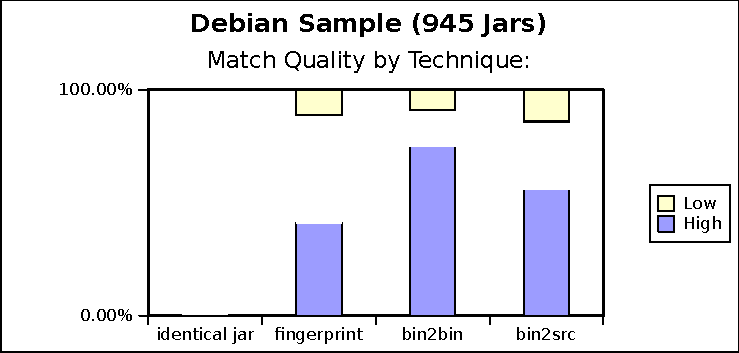
\includegraphics[width=\columnwidth]{plots/debianMatchQuality.pdf}
\end{minipage}
\hspace{0.5cm}
\begin{minipage}[b]{0.5\linewidth}
\centering
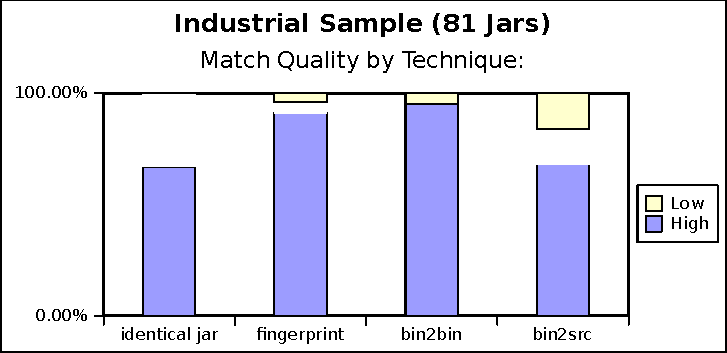
\includegraphics[width=\columnwidth]{plots/industryMatchQuality.pdf}
\end{minipage}
\vspace{-2mm}
\caption{A comparison of match quality by data set.  Left: Debian's 945
    jars.  Right: Industry's 81 jars.  The Industry set receives a boost of
    77\% binary-identical matches compared to Debian's 21\%.  Aside from
    this boost, the results appear similar.}
\label{fig:matchQuality}
\end{figure}


\subsection{Results II:  Industry Case Study, A Replication}

\begin{table}[h]
  \centering
\begin{tabular}[htbp]{l|r|lll|rrr}
  sha1-of-class/Industry-81  &              & \multicolumn{3}{c|}{\textbf{Similarity}}  & \multicolumn{3}{c}{\textbf{\# of Ties}} \\
  \textbf{Type of Match}     & Count        & Min   & Mdn    & Max   & Min  & Mdn  & Max  \\
  \hline
%& & & & & & & \\
  \emph{HQ1.} Exact (sha1 of jar)        & 54           & 1.0   & 1.0    & 1.0   & 1    & 2    & 14   \\
  \emph{HQ2.} Exact (sha1 of *.class)    &  9           & 1.0   & 1.0    & 1.0   & 1    & 1    &  5   \\
  \emph{HQ3.} Expected match             &  4           & 0.006 & 0.758  & 0.965 & 1    & 1.5  &  4   \\
  \emph{HQ4.} Version off by final digit &  7           & 0.016 & 0.500  & 0.962 & 1    & 1    & 12   \\
  \emph{\textbf{High Quality Matches}}   & \textbf{74}  &       &        &       &      &      &      \\
& & & & & & & \\
  \emph{LQ1.} Version off by many digits &  1           & 0.038 & 0.038  & 0.038 & 1    & 1    &  1   \\
  \emph{LQ2.} Not useful                 &  2           & 0.002 & 0.031  & 0.059 & 1    & 1    &  1   \\
  \emph{\textbf{Low Quality Matches}}    & \textbf{3}   &       &        &       &      &      &      \\
& & & & & & & \\
  \emph{\textbf{No Matches}}             & \textbf{4}   &       &        &       &      &      &      \\
%& & & & & & & \\
  \hline
  \textbf{Total Matches:} \hspace{3em}   \textbf{(95\%)} &  \textbf{77}   & \multicolumn{3}{c|}{\textbf{Average: 0.903}}  & \multicolumn{3}{c}{\textbf{Average: 2.8}} \\
   \multicolumn{8}{c}{} \\
   \multicolumn{8}{c}{} \\
  bin2bin/Industry-81        &              & \multicolumn{3}{c|}{\textbf{Similarity}}  & \multicolumn{3}{c}{\textbf{\# of Ties}} \\
  \textbf{Type of Match}     & Count        & Min   & Mdn    & Max   & Min  & Mdn  & Max  \\
  \hline
%& & & & & & & \\
  \emph{HQ1.} Exact (sha1 of jar)        & 54           & 1.0   & 1.0    & 1.0   & 1    & 3    & 16   \\
  \emph{HQ2.} Exact (sha1 of *.class)    &  9           & 1.0   & 1.0    & 1.0   & 1    & 1    &  9   \\
  \emph{HQ3.} Expected match             &  6           & 0.933 & 0.994  & 1.0   & 1    & 1    &  2   \\
  \emph{HQ4.} Version off by final digit &  8           & 0.133 & 0.915  & 1.0   & 1    & 1    & 12   \\
  \emph{\textbf{High Quality Matches}}   & \textbf{77}  &       &        &       &      &      &      \\
& & & & & & & \\
  \emph{LQ1.} Version off by many digits &  1           & 0.132 & 0.132  & 0.132 & 1    & 1    &  1   \\
  \emph{LQ2.} Not useful                 &  3           & 0.002 & 0.023  & 0.068 & 1    & 1    &  1   \\
  \emph{\textbf{Low Quality Matches}}    & \textbf{4}   &       &        &       &      &      &      \\
& & & & & & & \\
  \emph{\textbf{No Matches}}             & \textbf{0}   &       &        &       &      &      &      \\
%& & & & & & & \\
  \hline
  \textbf{Total Matches:} \hspace{2.5em} \textbf{(100\%)} & \textbf{81}  & \multicolumn{3}{c|}{\textbf{Average: 0.926}}  & \multicolumn{3}{c}{\textbf{Average: 3.6}} \\
   \multicolumn{8}{c}{} \\
   \multicolumn{8}{c}{} \\
  bin2src/Industry-81                    &              & \multicolumn{3}{c|}{\textbf{Best Match Score}}  & \multicolumn{3}{c}{\textbf{\# of Matches}} \\
  \textbf{Type of Match}                 & Count        & Min   & Mdn    & Max   & Min  & Mdn  & Max  \\
  \hline
%& & & & & & & \\
  \emph{HQ1.} Exact (sha1 of jar)        & \multicolumn{1}{c|}{\emph{n/a}} & & \emph{n/a} & & & \emph{n/a} &  \\
  \emph{HQ2.} Exact (sha1 of *.class)    & & & & & & & \\
  \emph{HQ3.} Expected match             &  41          & 0.168 & 1.0    & 1.0   & 1    & 1    &  2   \\
  \emph{HQ4.} Version off by final digit &  14          & 0.054 & 0.865  & 1.0   & 1    & 1    & 12   \\
  \emph{\textbf{High Quality Matches}}   & \textbf{55}  &       &        &       &      &      &      \\
& & & & & & & \\
  \emph{LQ1.} Version off by many digits &  12          & 0.061 & 0.491  & 1.0   & 1    & 1    &  1   \\
  \emph{LQ2.} Not useful                 &   1          & 0.068 & 0.068  & 0.068 & 1    & 1    &  1   \\
  \emph{\textbf{Low Quality Matches}}    & \textbf{13}  &       &        &       &      &      &      \\
& & & & & & & \\
  \emph{\textbf{No Matches}}             & \textbf{13}  &       &        &       &      &      &      \\
%& & & & & & & \\
  \hline
  \textbf{Total Matches:} \hspace{3em}    \textbf{(84\%)} &  \textbf{68}   & \multicolumn{3}{c|}{\textbf{Average: 0.812}}  & \multicolumn{3}{c}{\textbf{Average: 1.5}} \\
\end{tabular}
  \caption{These three sub-tables show the results from our industrial case
      study replication based on 81 open source jars.}
  \label{tab:bank}
\end{table}

Table~\ref{tab:bank} shows the results of our three matching techniques for
the replicated case study.  The 81 e-commerce jars represent a close
approximation of those found in a proprietary web application.  All 81 were
downloaded from original open source project websites directly, or if such was not
possible, they were built from tagged VCS versions.
Figure~\ref{fig:matchQuality} shows these results alongside the results of
the Debian experiment.

A close look at some of the \emph{HQ4} matches from the case study revealed
the data set includes library versions missing from the corpus's
collection.  Table~\ref{tab:close} shows these in detail.  Unfortunately,
two scenarios show that some jar versions will probably never be found in
any corpus:

\begin{enumerate}

\item The application developers may choose to use an experimental or
    ``pre-released'' version of a library that is unlikely to appear in any
    formal corpus.  We observed one example of this in our study
    (stax-ex-1.2-SNAPSHOT.jar).

\item Developers may download libraries directly from an open source
    project's version control system, for example, should they require a
    bleeding edge feature or a particularly urgent fix.  In these cases the
    jar is built directly from the VCS instead of from an official released
    version.

\end{enumerate}


\begin{table}[htbp]
  \centering
  \begin{tabular}{lll}
    \textbf{Correct jar}      &                & \textbf{Close match} \\
    \textbf{(not in corpus)}  & \textbf{Sim}  & \textbf{(from corpus)} \\
\hline\hline
                      jaxws-api-2.1.3.jar & 1.0 & jaxws-api-2.1.jar       \\
                 stax-ex-1.2-SNAPSHOT.jar & 1.0 & stax-ex-1.2.jar         \\
                     streambuffer-0.5.jar & 1.0 & streambuffer-0.7.jar    \\
\hline
  \end{tabular}
  \vspace{1mm}
  \caption{Three matches with similarity=1 were close in version to the correct (missing) jars.}
  \label{tab:close}
\end{table}




For $44$ of the $81$ binary jars ($54\%$), our method found several
candidates in the corpus that tied for best similarity score of $1.0$.  In
all cases the candidate set covered a contiguous sequence of versions, as
shown in Table~\ref{tab:contiguous}, save for holes in the corpus's
collection.  Of these $44$ tied matches, the exact match was present for
$42$ cases.  The remaining two cases, \mytt{xpp3\_min-1.1.4.jar} and
\mytt{sun-jaxws-2.1.3-20071218-api.jar}, we classified as \emph{HQ4}
matches.  In both cases an exact match was not present in the corpus.

\begin{table}[htbp]
  \centering
  \begin{tabular}{rl}
    \textbf{Similarity to}  & \\
    \textbf{asm-attrs-2.2.3.jar}  &  \textbf{Artifacts from corpus}\\
\hline\hline
                 1.0 & asm-attrs-2.1.jar    \\
                 1.0 & asm-attrs-2.2.jar    \\
                 1.0 & asm-attrs-2.2.1.jar  \\
                 1.0 & asm-attrs-2.2.3.jar  \\
\hline
  \end{tabular}
  \vspace{1mm}
  \caption{Example of multiple matches with similarity=1.  The
    exact match is asm-attrs-2.2.3.jar.}
  \label{tab:contiguous}
\end{table}

In general the results are similar to our Debian experiment, except in one
respect.  Less then 0.3\% of the Debian sample are identical jar copies
(\emph{HQ1}).  Whereas in this data set of archives downloaded directly
from project websites, rather than recompiled by Debian, the number of
identical copies (\emph{HQ1}) stands at 54 (67\%), with another 9 (11\%)
identical contents matches (\emph{HQ2}).  This suggests fingerprint
approaches may be particularly useful in industry settings, at least for
binary-to-binary matching.  This may be for two reasons.  First, Maven
appears to often contain identical copies to those located on the upstream
project websites, and industry developers may be directly downloading
dependencies from the project sites.  Second, industry may be using the
Maven repository to resolve their dependencies, anyway.

Another small difference arises in the binary-to-source results.
These results do not receive any benefit from the ``binary-identical
boost'' described in Figure~\ref{fig:matchQuality}, and yet the
high-quality matches (\emph{HQ3} to \emph{HQ4}) comprise 68\% of the total,
noticeably higher than the 56\% found in the Debian sample.
We also note that all of our
provenance techniques, including the simple baseline approaches, enjoyed
improved performance when used on the e-commerce jars.

We can also compare the results of our replication against the original
results from our previous report.  Compared to the previous report
we were able to achieve one additional match (since the artifact, \mytt{chiba.jar},
had since appeared in Maven), and in several cases the cardinality of top-matching
ties were reduced.   The example shown in Table~\ref{tab:improvement}, \mytt{wicket-ioc-1.4.0.jar},
was the most dramatic reduction in top-matching ties, from 31 ties in our 2011 paper,
compared with 11 ties in this paper.  By reducing the number of
top-matching ties, we reduce the amount of additional work end-users of our tools
must employ after-wards, in order to further refine their results to a single match.

\begin{table}[htbp]
  \centering
  \begin{tabular}{|r|r|r|}
\multicolumn{3}{l}{\textbf{Similarity Scores for Case Study (2011) \& Replication (2012)}} \\
\multicolumn{3}{l}{\emph{Comparing results for \mytt{wicket-ioc-1.4.0.jar}}} \\
\hline
 & & \\
\textbf{Top Matches}       & \emph{2011}   & \emph{2012} \\
\hline
wicket-ioc-1.3.0-beta2.jar & 1.000  &  0.538 \\
wicket-ioc-1.3.7.jar       & 1.000  &  0.538 \\
wicket-ioc-1.4-rc1.jar     & 1.000  &  1.000 \\
\textbf{wicket-ioc-1.4.0.jar} & 1.000  & 1.000 \\
wicket-ioc-1.4.3.jar       & 1.000  &  1.000 \\
wicket-ioc-1.4.8.jar       & 1.000  &  0.667 \\
                           &        &        \\
\emph{[etc... 26 additional top-ranked 1.000} & & \\
\emph{matches in 2011 case-study omitted]} & & \\
\hline
\multicolumn{1}{|r|}{~~~~~~~~~~~~~\textbf{Total \# of Top-Ranked Tied Matches:}} & 31 & 11 \\
\hline
  \end{tabular}
  \vspace{1mm}
  \caption{Here we compare a single result from
our original 2011 case-study \cite{DaviesGGH11}
against the same result in this 2012 replication.
With our improved signature-extraction tool,
we are able to narrow the number of ties
reported back for \mytt{wicket-ioc-1.4.0.jar}
from 31 ties down to 11 ties.
Similarity scores tend to drop off faster
as versions diverge when we analyze jars using our newer signature-extractor.}
  \label{tab:improvement}
\end{table}



\subsection{Summary of Results}

\subsubsection{RQ1, \rqOne}

\textbf{RQ1:}
The similarity index is highly useful at narrowing the search space to find
original \emph{binary} archives, as is the fingerprint index.  In fact, the
baseline fingerprint approach produces even narrower search spaces (e.g., 2.4 ties per
result on average compared to 3.5).  But the narrower search space comes
with a cost of reduced recall.  This trade-off lies at the heart of
Bertillonage.  In our study we considered two index approaches:
byte-oriented, and Bertillonage-oriented.  Both approaches have important
benefits.  For example, with the byte-oriented approaches, a 1.0 match is
authoritative, whereas with our signature techniques (and presumably any
Bertillonage approach), even a 1.0 match could be false, insomuch as
provenance is concerned.  Since performance and storage costs imposed by
each index are relatively small (both in index creation, and query
execution), a hybrid approach would not impose undue resource or performance costs.
By adopting a hybrid approach, implementors can benefit from the
certainty offered by the byte oriented approaches, while also enjoying the
improved recall and superior match quality we observed in our Bertillonage approaches.


\subsubsection{RQ2, \rqTwo}

\textbf{RQ2:}
The similarity index is useful the majority of the time to narrow the
search space to find original \emph{source} archives, although we observed
inferior performance compared to binary-to-binary matching.  We suspect two
factors are contributing to the inferior performance.


First, our corpus contains only $1,650,000$ Java source files
compared to $2,430,000$ compiled class files.  This results in fewer
source archives available for matching.  For example,
\mytt{batik-util-1.6.jar} matched no source archives, and yet for RQ1 the
same jar file matched $23$ distinct binary archives, ranging from
similarity $1.0$ down to $0.005$.  Second, fundamental problems about
source archives pose difficult obstacles in this area.  We often assume a
simple 1-for-1 mapping between sources files and binary files, but the
reality is more complex.  Techniques such as unit tests, code generation,
bytecode manipulation can thwart the 1-for-1 assumption.  Also, metrics
based on set similarity have a hard time when build scripts produce several
small binaries instead of a single large one.

To conclude, our bin2src experiment suggests we can match the sources the
majority of the time, even with an inferior corpus.  In future work we
envision employing a better corpus (with fewer holes) so we can better
isolate the fundamental problems of binary-to-source matching.




%In RQ1 we propose a hybrid approach, perhaps we can offer the same suggestion here:
%      binary provenance bridging.  The binary-to-binary techniques often perform very well,
%      and once binary provenance information is obtained, locating a project's website, and downloading
%      the corresponding source code may very well be a simple, straighforward, and ultimately
%      much more robust technique compared
%      to any automatic and direct techniques.



\subsubsection{RQ3, \rqThree}
\label{sec:mavenreliability}

To address RQ3 we took two snapshots of the Maven repository and checked to
see how reliable the file-name could convey the version information of the
archives.  We explored the Maven corpus to see if any jars were mislabelled
or were duplicates. We did this by a bitwise comparison of the jar files to
each other and checking for inconsistent file names. $99.1\%$ of the jars
were unique.  $0.83\%$ of the corpus was exact duplicates, that is there
were multiple names for the same file.  Of the exact duplicated $30.7\%$
did not share the same project name.  Most of these have some version
numbering but are not consistently named (abbreviations, license
annotations). Many files are identical with different names because there
was no change in that archive between versions. 

We compared snapshots of Maven at two different times: June 15, 2010 and
July 30, 2011. We found that the reliability of Maven had increased by by
$0.03\%$ in terms of duplication.  Our first Maven snapshot had $0.86\%$
exact duplicates while our last snapshot had $0.83\%$ exact duplicates,
this reduction of $0.03\%$ was a statistically significant difference
(Student T-test p-value $< 0.001$).  Thus Maven's reliability as an
authoritative repository has increased over time. Yet, we have demonstrated
that even in a carefully curated repository such as Maven, there can be
some version ambiguity.

\vspace{-2mm}

\subsection{How Fast Are The Techniques?}
\label{perf}

\vspace{-1.6em}

\begin{table}[h]
  \centering
\begin{tabular}[htbp]{r|r|r|l}
\multicolumn{4}{l}{\textbf{Source-to-source analysis of \mytt{commons-collections-3.2.1-src.zip}}} \\
\multicolumn{4}{l}{\textbf{(with $a=469$) executed in 6.169 seconds:}} \\
\multicolumn{4}{l}{ } \\
\hline
\emph{$b$} & \emph{$a \bigcap b$} & \emph{similarity} & \emph{provenance candidates} \\
\hline
   73 &            19 &  0.036  & commons-collections-2.1-sources.jar \\
   76 &            19 &  0.036  & commons-collections-2.1.1-sources.jar \\
  249 &           112 &  0.185  & commons-collections-3.0-sources.jar \\
  268 &           201 &  0.375  & commons-collections-3.1-sources.jar \\
  \textbf{469} & \textbf{469} &  \textbf{1.000}  & \textbf{commons-collections-3.2-src.zip} \\
  274 &           274 &  0.584  & commons-collections-3.2-sources.jar \\
  274 &           274 &  0.584  & commons-collections-3.2.1-sources.jar \\
\multicolumn{4}{l}{ } \\
\emph{$b$} & \emph{$a \bigcap b$} & \emph{similarity} & \emph{clone candidates} \\
\hline
 1925 &           274 &  0.129  & openjpa-all-2.0.0-sources.jar \\
 1925 &           274 &  0.129  & openjpa-all-2.0.1-sources.jar \\
 2326 &           274 &  0.109  & openjpa-all-2.1.0-sources.jar \\
  101 &             4 &  0.007  & commons-beanutils-1.8.0-sources.jar \\
  101 &             4 &  0.007  & commons-beanutils-1.8.1-sources.jar \\
  101 &             4 &  0.007  & commons-beanutils-1.8.2-sources.jar \\
  101 &             4 &  0.007  & commons-beanutils-1.8.3-sources.jar \\
  300 &             4 &  0.005  & prettyfaces-jsf2-3.2.1-sources.jar \\
  300 &             4 &  0.005  & prettyfaces-jsf2-3.3.0-sources.jar \\
\end{tabular}
  \caption{
This analysis
of \mytt{commons-collections-3.2.1-src.zip}, a Java source archive
containing 58,000 lines of code, completed in
6.169 seconds on an Intel core-i3 laptop, 
The top match is an ``\emph{HQ2}'' match:
the expected version number is off by one digit (3.2 instead of 3.2.1).
%The analysis identified \mytt{commons-collections-3.2.1-sources.jar} as an imperfect match (similarity = 0.584),
%despite an exact version match in the name of the archive.
%This lower match is because \emph{-sources.jar} files, as opposed to a \emph{-src.zip} archives,
%do not include JUnit tests, and thus contain fewer class signatures.
These results help us roughly compare performance
against Livieri et al.'s D-CCFinder \cite{LivieriHMI07}, where
analysis of a 47,000 line C project was analyzed in 40 minutes
using 80 Pentium IV computers running in parallel (in 2006).
We believe our results and performance numbers make a strong
case for software Bertillonage as an effective \emph{initial} approach for clone and provenance
analysis.}
  \label{tab:src2src}
\end{table}




One of the primary goals of software Bertillonage is to employ fast, light-weight, and approximate
techniques to quickly narrow searches for provenance.
In other words, software Bertillonage queries should take seconds rather than hours.
We compare our approach's performance to D-CCFinder's 2006 result \cite{LivieriHMI07},
since D-CCFinder illustrates state-of-the-art performance characteristics of exhaustive
clone-detection.
Livieri et al. performed two experiments in their paper.  In the 1st experiment
they analysed the complete FreeBSD project for code-cloning between sub-modules.
In the 2nd experiment they indexed the FreeBSD project, and then analyzed a separate,
smaller project, SPARS-J, to see if any of SPARS-J's code could be traced back to FreeBSD.
The 2nd experiment is of interest to us, since the aims, design, and execution
of that experiment are similar to our own, although they employ source-to-source
analysis exclusively, whereas our tools also allow binary-to-binary, binary-to-source, and source-to-binary
analysis.

SPARS-J's source code contained 47,000 lines of C code.  D-CCFinder's analysis
ran in 40 minutes using a customized verison of CCFinder distributed to 80 Pentrium IV 3.0ghz workstations
in a university lab, each configured with 1GB of RAM.
Our own tools ran on a single dual-core Intel Core i3 2.26 GHz
laptop with 8GB of RAM.
To roughly compare our performance against the D-CCFinder result, we ran source-to-source
analysis using \mytt{commons-collections- 3.2.1-src.zip}, which contains 58,000 
lines of Java code, and thus can be considered similar to SPARS-J in terms
of size.   Uncompressing the source archive required 0.171 seconds.   Signature extraction of the sources
required 5.275 seconds.  Running the query took 0.723 seconds.  In total the analysis
required 6.169 seconds.  The results of
the query are shown in Table~\ref{tab:src2src}.
This small example illustrates software Bertillonage's strengths:  useful results
are found quickly from within a massive set of possible matches.  But the results also
can require further analysis:  in this case separating the results into ``provenance candidates''
and ``clone candidates'' required human expertise; and realizing that the \mytt{3.2.1-sources.jar}
match does not contain JUnit tests, whereas the \mytt{3.2-src.zip} archive does (improving its similarity score),
also required additional analysis.

We also collected performance data on our indexing of Maven2, as well as our experiments
on the Debian and E-Commerce Jars.   Our aim in collecting this data was simply
to show that \emph{anchored class signatures} are fast enough to be very usable in almost all cases
we encountered!  We are not trying to prove
any particular run-time complexity of our approach, since the queries involved
are straight-forward database lookups.

As Table~\ref{tab:sigCreationSpeed} suggests, scanning the complete Maven2
repository on the laptop would require 6 hours to scan the 7,140,000 source
files, and 1.5 hours to scan the 19,780,000 binary files (our current
toolset does not skip duplicates).  The binary
fingerprint scan would require 20 minutes.  The reality, however, is
slower, since these rates do not include time required to decompress
\emph{zip}, \emph{jar}, and \emph{.tar.gz} archives\footnote{Unfortunately, we did not instrument our tools to collect unzip timings.}.
The time required to
generate queries is similarly affected by these rates, since each signature
in the query must be first extracted from the subject archive.

%As one
%would expect, query generation is linear with respect to the number of
%classes being scanned.


\begin{table}[h]
  \centering
\begin{tabular}[htbp]{l|r@{}l@{}l}
\textbf{Signature Type}   & \multicolumn{3}{c}{\textbf{Creation Rate, Non-Compressed Files}} \\
\hline
fingerprint, SHA1                         & $15,250 / sec~$ & $\times 19,780,000$ & $~= ~~22 ~mins$ \\
anchored class signature, Java bytecode   & $ 3,450 / sec~$ & $\times 19,780,000$ & $~= ~~96 ~mins$ \\
anchored class signature, Java source     & $   330 / sec~$ & $\times ~7,140,000$ & $~= ~361 ~mins$ \\
\end{tabular}
  \caption{
The time it takes to index a corpus, as well as the time needed to generate subsequent queries,
depends partly on the rate at which signatures can be generated.  As this table shows,
anchored class signatures for source files are the slowest to create.  Maven
contains 19,780,000 class files and 7,140,000 source files.
  }
  \label{tab:sigCreationSpeed}
\end{table}


To help us understand our performance data we developed a very simple
model that we believe represents a lower-bound on the amount of work
the database must perform:

\begin{enumerate}

\item Each signature in the query must be examined against the database's ``signature'' index.

\item Each row in the output must be examined against the database's ``archive'' index.

\end{enumerate}

Presumably the database performs a large amount of intermediate work inbetween these two stages joining
various tables and sub-selects, but this simple model allows us to visualize the
performance information we are most interested in:  1.) How big is the Jar file we are analyzing?  2.) How many matches
did we find? and 3.) How long did it take?
Table~\ref{tab:perfSummary} presents aggregates of our performance data using this model,
and Figures~\ref{fig:perfBin2Bin3quartiles} and \ref{fig:perfBin2Bin}
provide a complete visualization.  We ran all experiments three times, and took an average timing
from the three runs.  On our laptop the 1st execution tended to run 4 times slower than subsequent executions; we suspect
this may be due an aggressive caching policy within the PostgreSQL database engine.
Since each run only executes approximately 4,000 queries, we suspect PostgreSQL is able to
cache significant portions of the results inbetween runs.


\begin{table}[h]
  \centering
\begin{tabular}[htbp]{l|rrr|rrr}
                                    & \multicolumn{3}{c|}{\textbf{Signatures + Results}}  & \multicolumn{3}{c}{\textbf{Seconds}} \\
  \textbf{Provenance Technique}     & Mdn   & Avg    & SD    & Mdn  & Avg  & SD  \\
  \hline
  fingerprints, sha1-of-jar         &  3.0  &   2.8  &   1.1 & 0.254  & 0.261  & 0.032   \\
  fingerprints, sha1-of-classes     & 57.0  & 151.8  & 258.4 & 0.405  & 0.558  & 1.058   \\
  signatures, bin2bin               & 79.0  & 188.8  & 290.6 & 0.286  & 0.674  & 1.483   \\
  signatures, bin2src               & 68.0  & 151.4  & 260.5 & 0.240  & 0.342  & 0.470   \\
  \hline
\end{tabular}
  \caption{Performance comparison of the 4 techniques processing all jars
    (945 Debian + 81 Industry).  All techniques
    performed very quickly, with bin2bin the slowest, requiring on average 2/3rds of a second 
    per jar analyzed.}

  \label{tab:perfSummary}
\end{table}




\begin{figure}[h]
  \centering
%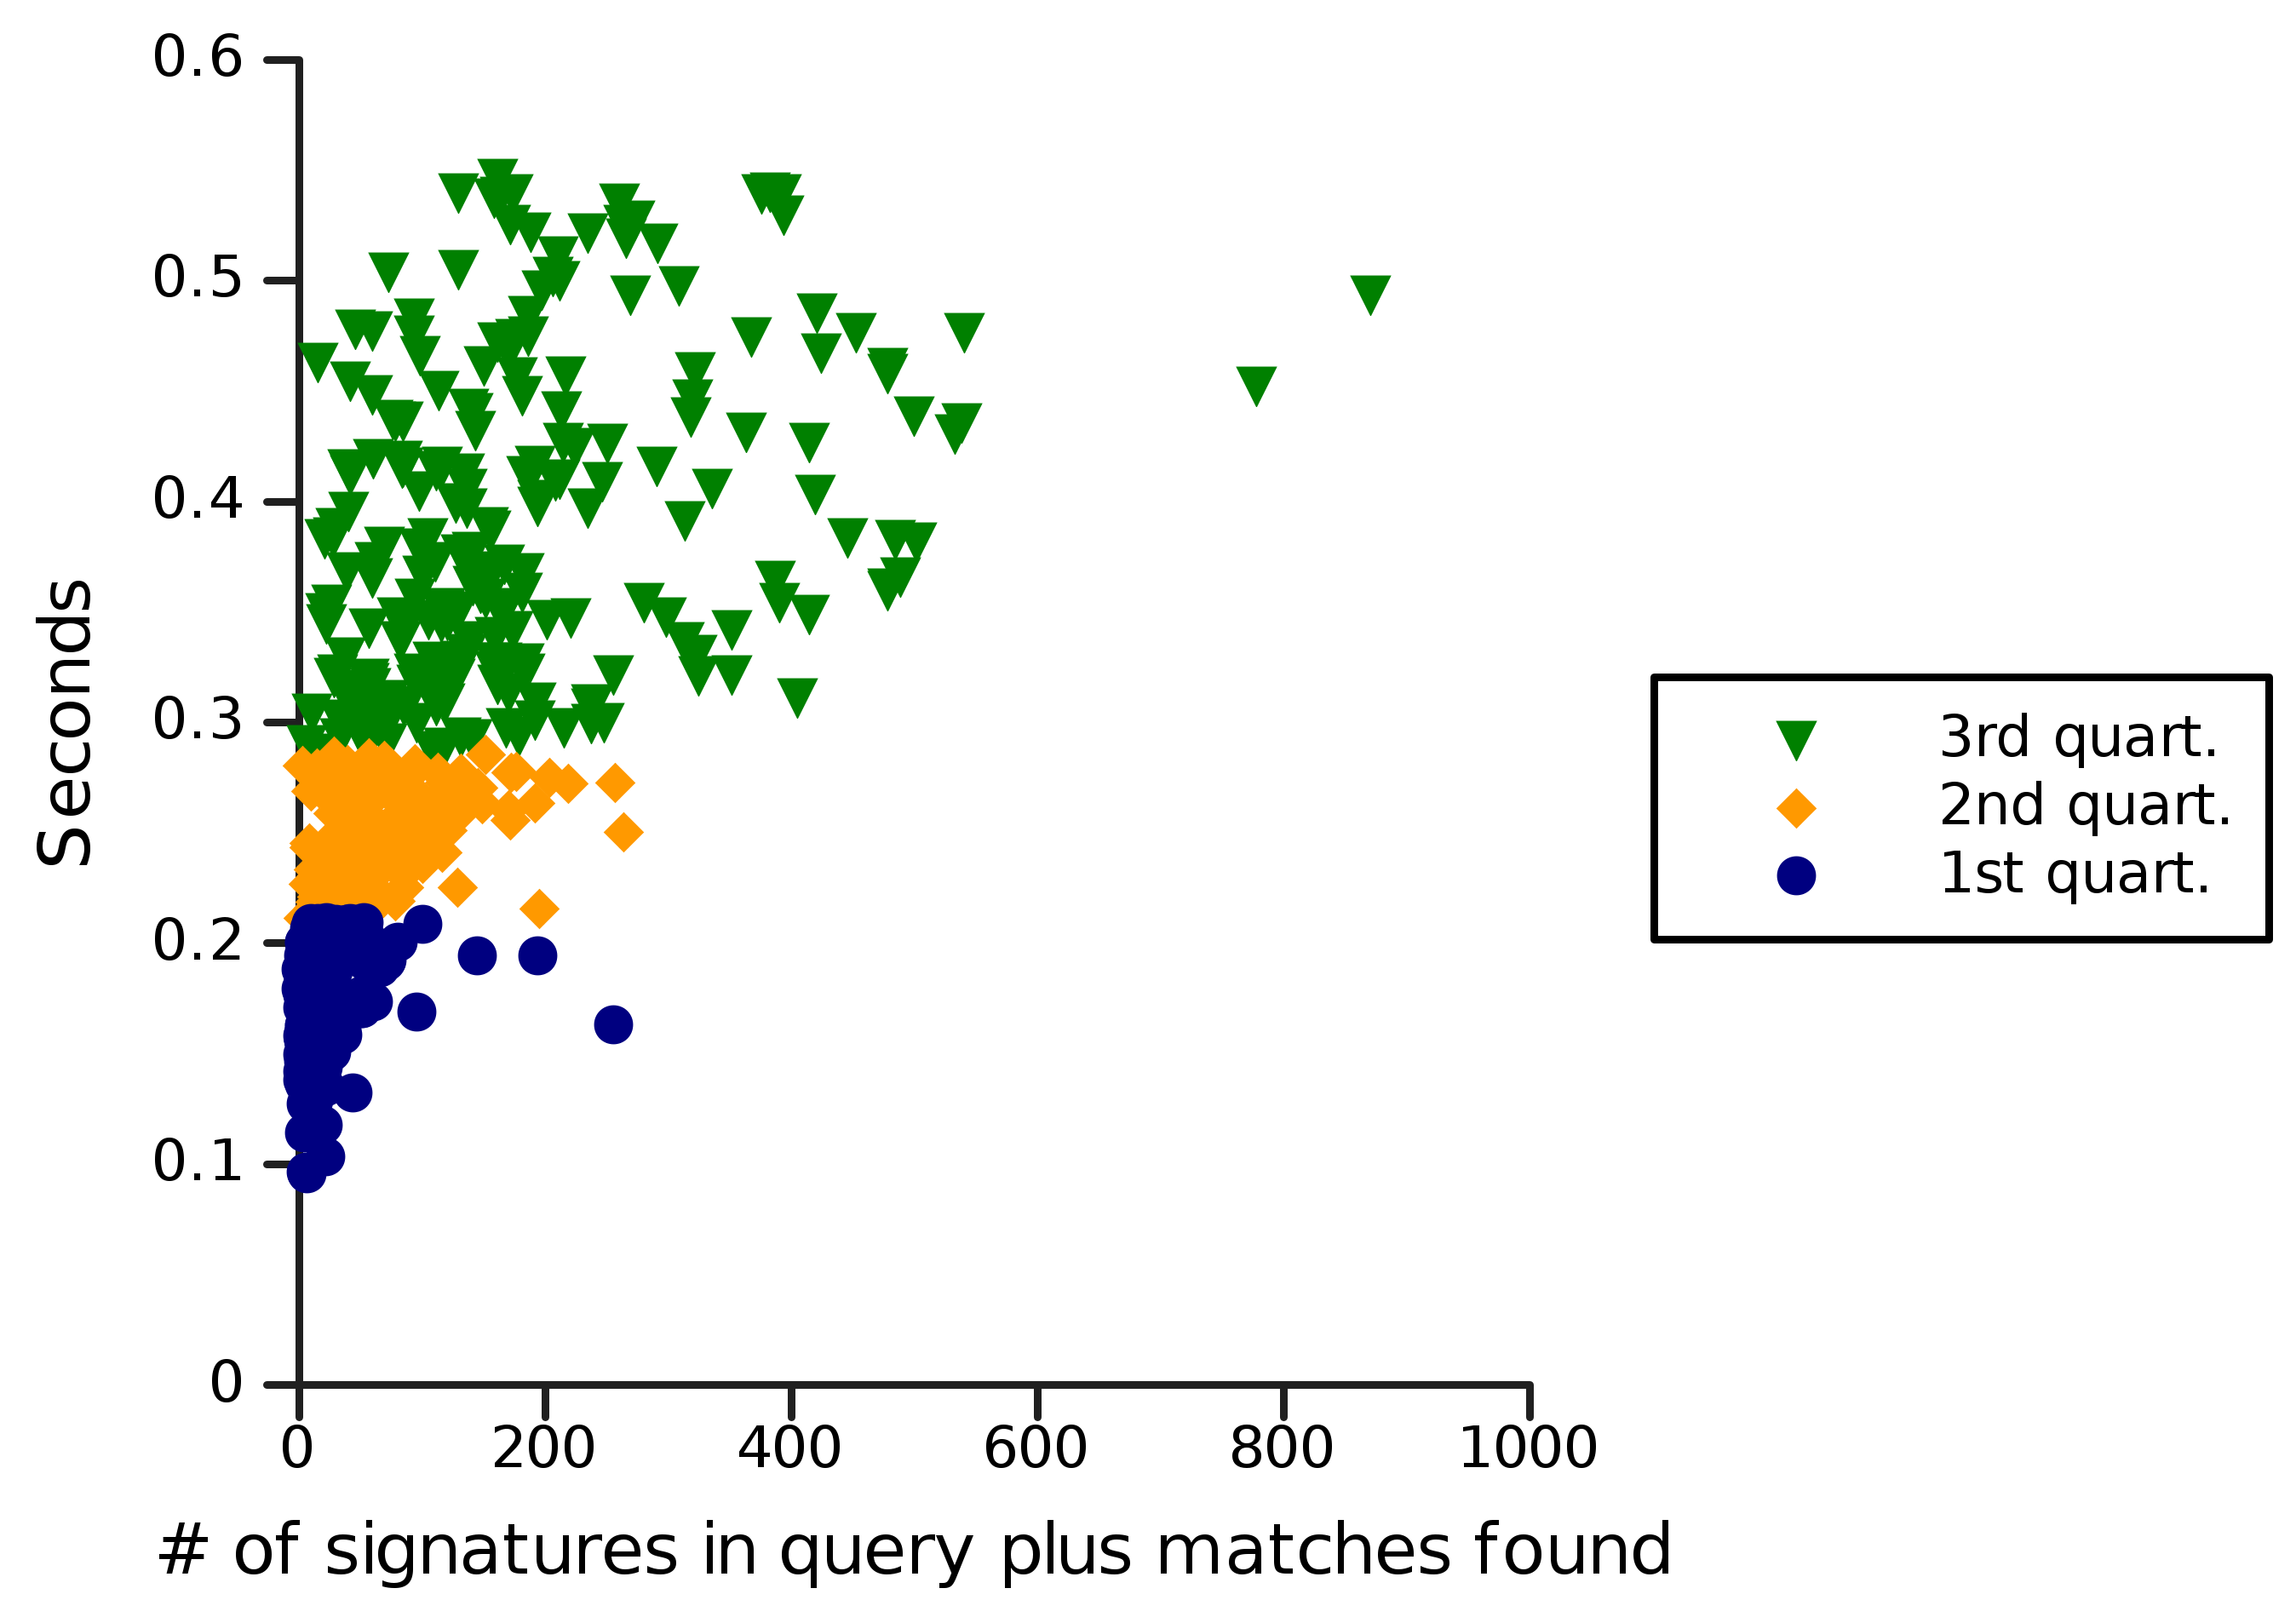
\includegraphics[width=40em]{plots/3quartiles.png}
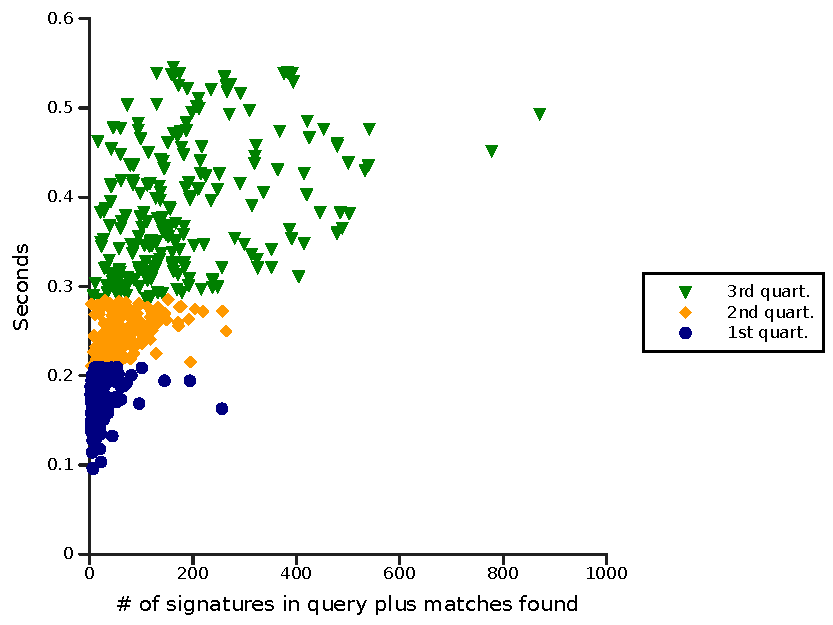
\includegraphics[width=40em]{plots/a.pdf}
  \caption{\small{A closeup on the fastest 75\% of the bin2bin queries (divided
    into quartiles), with q1=fastest, q2=medium fastest, and q3=medium
    slowest.  We plot execution time against a combined tally of results
    returned plus the \# of signatures in the query.  The tally
    models a useful lower-bound on amount of work the database needs to perform.}
}
  \label{fig:perfBin2Bin3quartiles}
\end{figure}
\begin{figure}[h]
  \centering
%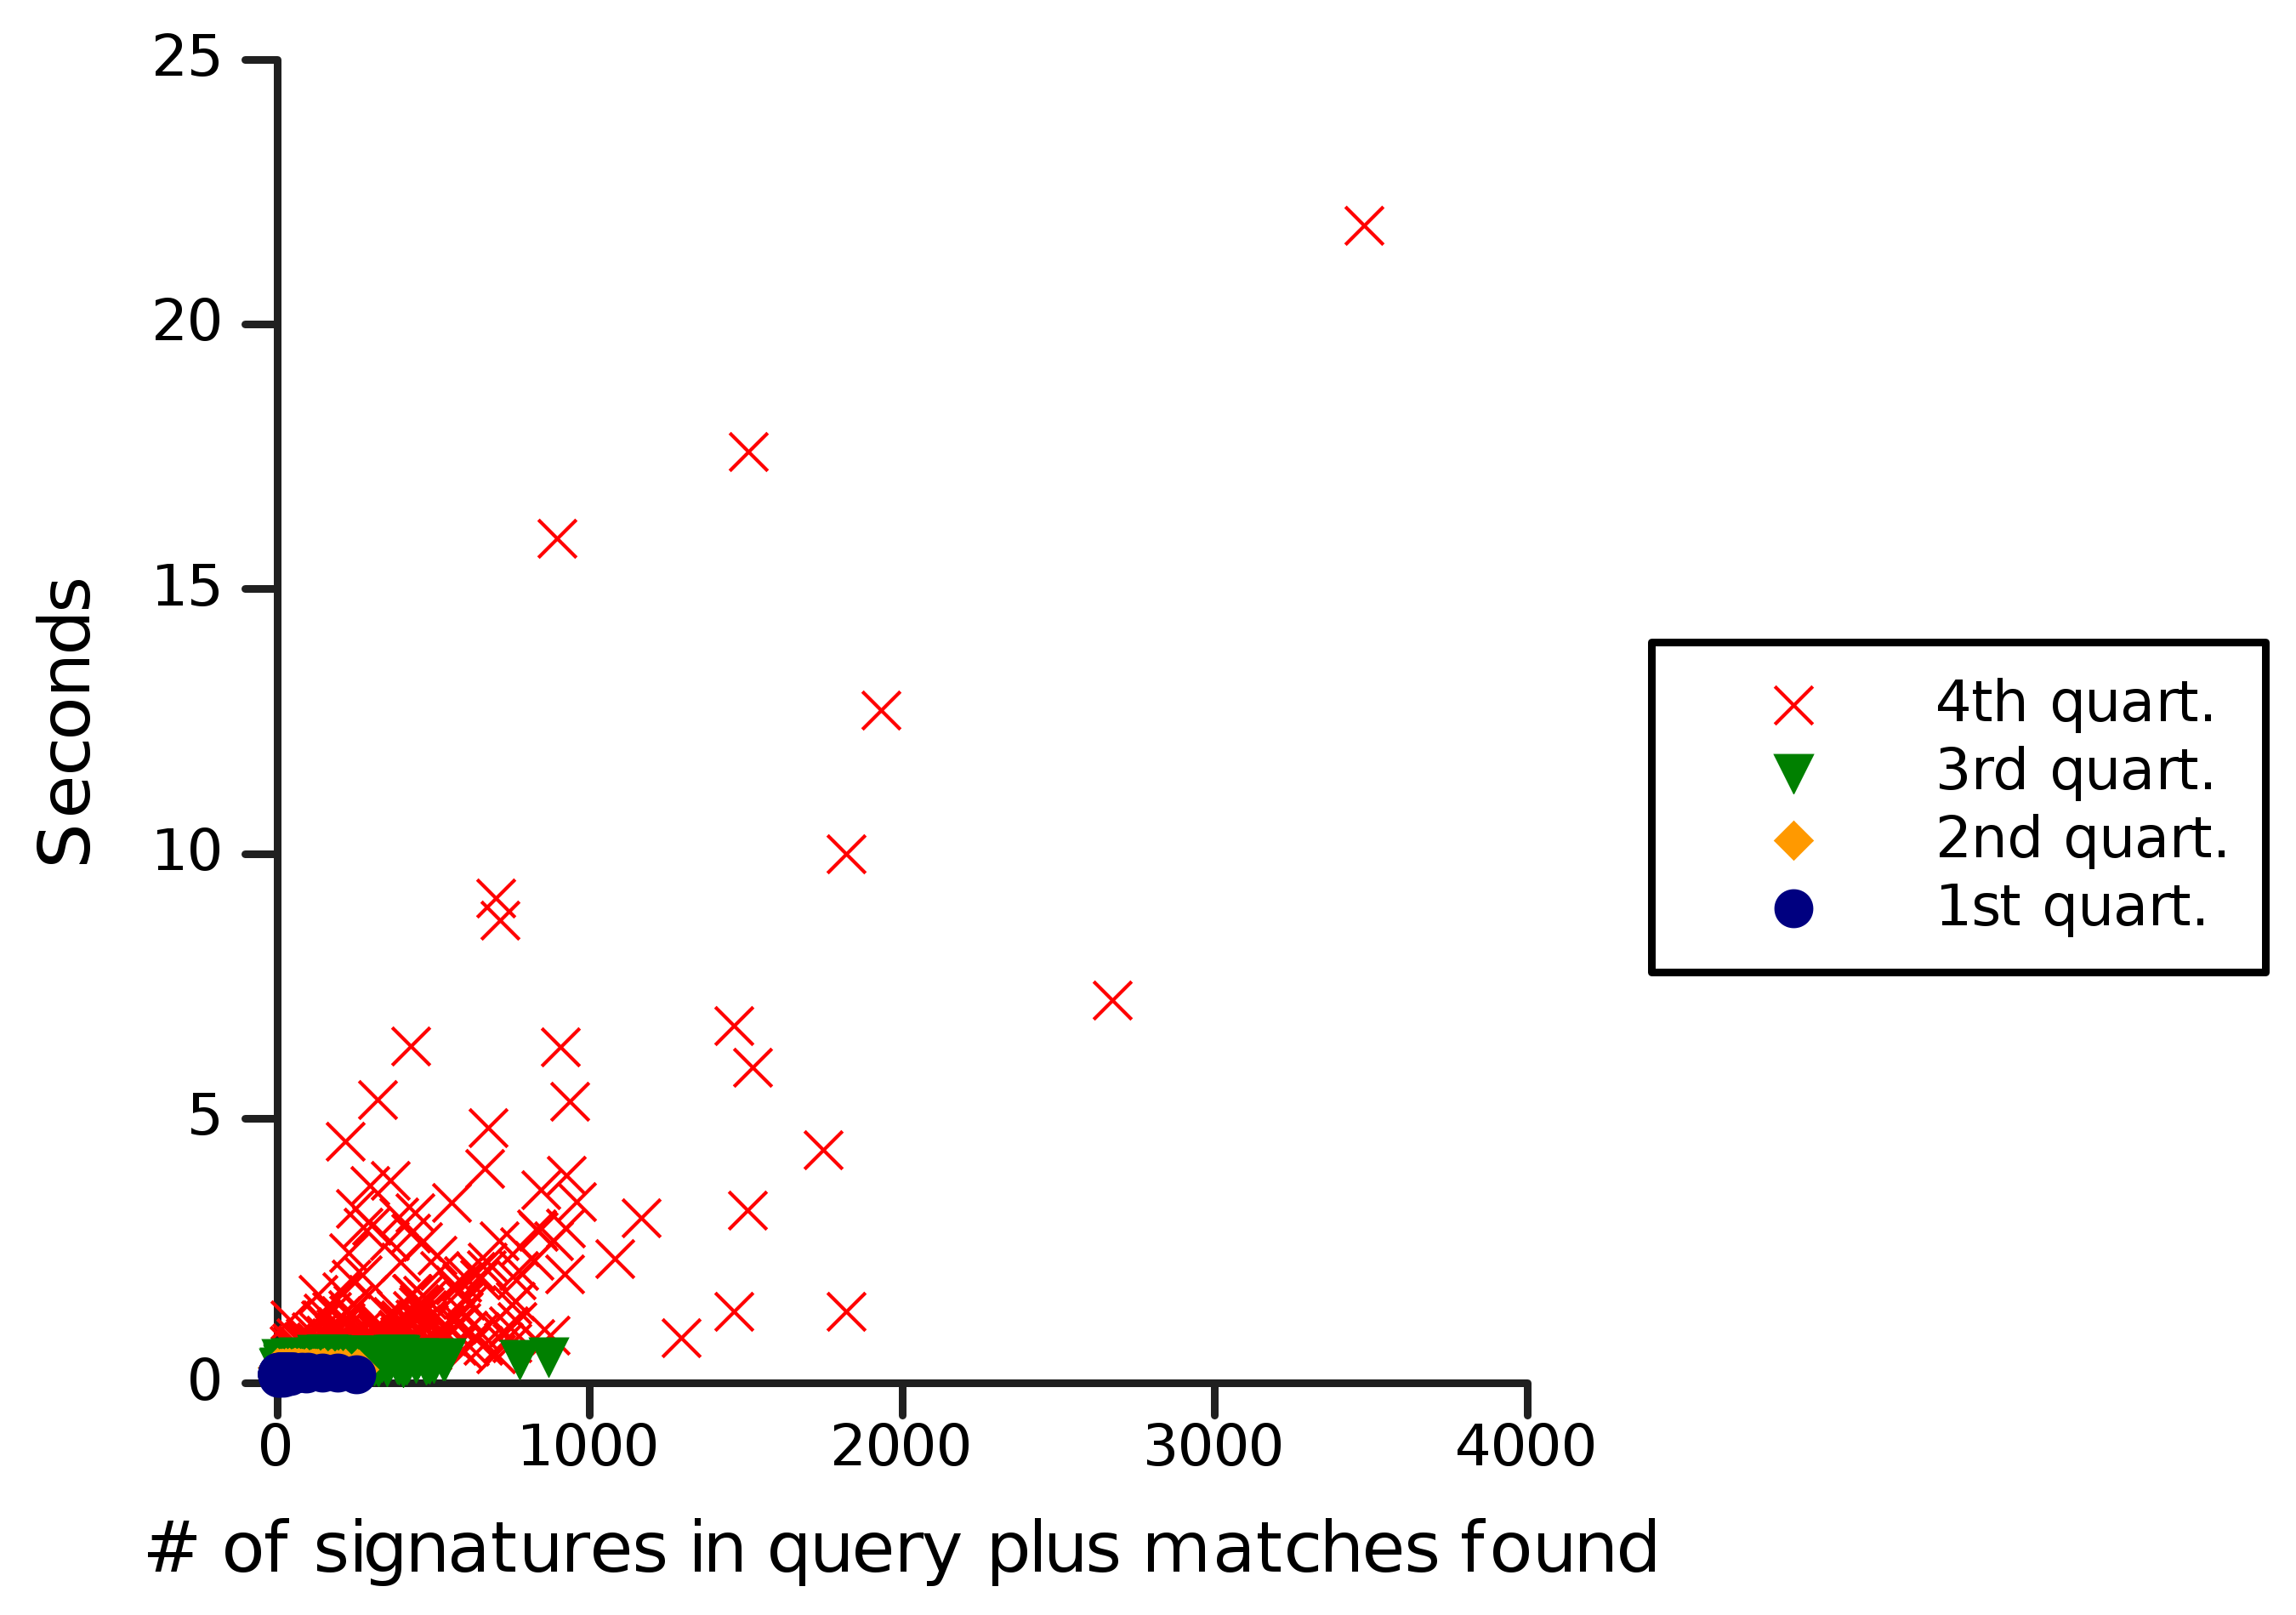
\includegraphics[width=40em]{plots/4quartiles.png}
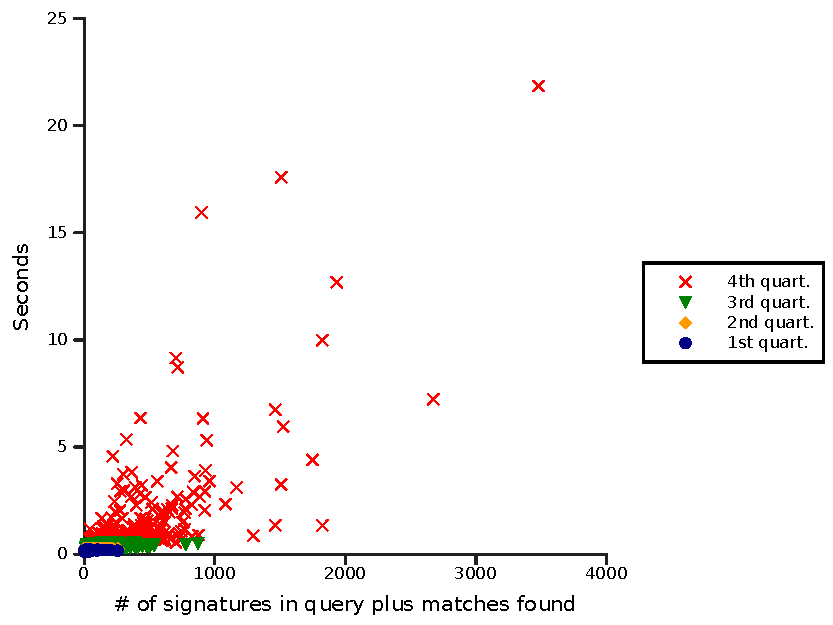
\includegraphics[width=40em]{plots/b.pdf}
\vspace{-2mm}
  \caption{\small{The wide-angle view of the bin2bin query performance (all four
    quartiles), with q1=fastest (barely visible), q2=medium fastest,
    q3=medium slowest, and q4=slowest.  We plot execution time against a
    combined tally of results returned plus the \# of signatures in the
    query.  The tally models a useful lower-bound the amount of work the database needs to
    perform.  The query for \mytt{aspectjtools-1.6.9.jar} in the case study
    took nearly 22 seconds to execute on average.  It contains 2,810
    signatures and its query returns 668 rows.}
}
  \label{fig:perfBin2Bin}
\end{figure}



To summarize, \emph{anchored class signatures} exemplify software Bertillonage:
they are simple, approximate, and significantly faster than exhaustive clone-detection
techniques.   And they are effective.  With most queries requiring on average 2/3rds of a second,
our \emph{anchored class signatures} implementation could be feasibly offered to programmers
within an Integrated Develompent Environment (IDE) such as Eclipse (e.g., right-click on a jar,  click Bertillonage...).
Thanks to previous exhaustive techniques, such as D-CCFinder, it was feasible for programmers,
researchers, and other stakeholders to
run clone-analysis against very large systems.  But they needed a strong case to justify the
time and resource utilization.  With faster light-weight Bertillonage methods, such as
the \emph{anchored class signatures} offered here, provenance analysis
can begin to support stakeholders who \emph{want to know}, as opposed to only those who \emph{need to know}.



%Index queries should perform similar to the Bertillonage techniques, since
%the query structure is identical, but in practice they run faster, due in part
%to the lower frequency of matches (e.g., 2.4 top matches per query compared to
%3.5 for bin2bin).  This makes sense, since any change to a source file,
%even a new comment (and in some cases, a different compiler),
%and certainly any code change, will perturb its
%compiled binary representation, in turn altering its fingerprint, and precluding
%the match.
%This stands in sharp contrast to the Bertillonage class signatures, which are only perturbed by functional
%changes ``outside the curly braces,'' and thus are subject to change by a much smaller set of 
%developer activities.



%\item Debian sample shows that an imperfect corpus can still provide many useful provenance answers.
%      The fact this Debian sample is arguably more challenging from a provenance perspective
%      than what we might expect to observe in nature further strengthens this claim.
%      (e.g., Debian patches sources, uses less common compilers, and has a policy of recompiling).

%\item The industry case study shows how the corpus's own context is important to consider,
%      independent of the corpus's completeness.
%      In this particular example, since the Maven2 repository serves as the main dependency
%      resolver for this particular company, by using the same pool from which the company is obtaining
%      its libraries, we significantly boost the power of the byte-oriented techniques.
%      We also wonder if the company is less likely to consider libraries not already present in Maven2,
%      since such are probably inconvenient for developers to integrate into their existing environments.
                                                                   
%\item Our bin2src experiment sheds some light on how an even further degraded corpus might
%      impact a provenance method.  Source signatures in Maven are 2 times less common, and
%      yet the results in our bin2src experiments were surprisingly decent.






%dmg's bin2src Results:

%\begin{itemize}
%\item 1 same name but .zip instead of .jar (Jaccard 1)
%\item 32 Same name, including -source (max 1.0, min 0.85, median 1.0)
%\item 7 variations of name. Max 1.0, min 0.609, median 0.952. For
%  example: sun-jaxws-2.1.4-20080502-rt and jaxws-rt-2.1.4;19;
%\item 23, variations of version.. We also checked the Inclusion in
%  this one: max 1.0, min 0.113, median 0.929). We checked every one
%  of them and they really looked like different variations in version
%  even those with the lowest Jaccard jdom-1.0.jar and
%  jgom-1.1-sources, with In. 113, and Jaccard .061, the lowest)
%\item 5 False positive (not matched): Min;0.068, Max;0.225,
%  Median;0.200, but even their inclusion is very  low: (Min;0.068,
%  Max;0.225, Median;0.186).
%\item 13 not found. 
%\item For 60, there was only 1 match, for the remainder 21, the min was 2, max, 11, with median of 3. Really narrowing the searching space.
%\item Results changed: now only 20 \emph{1.00} match is a single match, but median for single match is 2
%\end{itemize}





%%% Local Variables: 
%%% mode: latex
%%% TeX-master: "000_main"
%%% End: 



%   We tried running our analysis against Google's android.jar, a jar not currently contained
%   in the Maven2 repository). Our method decided
%   it must come from Sun/Oracle's jdk sources (jdk-6u20-ea-src-b02-jrl-01\_apr\_2010.zip)
%   with 221 matches.
%   Together with the cayenne-1.2.2.jar results in Table \ref{tab:falseMatch},
%   this shows how our method becomes confused by large clone imports,
%   since these cause a spike in secondary matches, potentially eclipsing the primary
%   matches.  In addition, there is no way for our method to reliably distinguish
%   between primary and secondary matches.  For all our method knows, cayenne-1.2.2 is
%   the canonical location for the commons-collections-3.1 classes, and not the other
%   way around.

%   But this confusion also has its uses:  Apache HttpClient developers recently
%   wanted to know what version of their libraries Google had statically imported
%   into the android.jar file.  By querying android.jar in our index we were
%   able to provide specific version information concerning two libraries published
%   by the Apache HttpClient team:  httpcore-4.0-beta2.jar, and httpclient-4.0-beta1.jar.
%   See Table \ref{tab:android} to see how these were identified.  The main HttpClient
%   developer asked if we could also test against httpclient-4\_0\_API\_FREEZE.jar,
%   an uncommon version he suspected Google had actually imported.  We loaded
%   httpclient-4\_0\_API\_FREEZE.jar into our index and re-ran the query with android.jar.
%   The match-count was the same, but the earlier zip-date caused our method to pick this,
%   certainly not contradicting the main developer's suspicion.  In this way our tool
%   serves as a useful clone detection engine, especially for static imports.


% ------Ties and License Resolution---------
%   One interesting
%   possibility arises when considering ties in conjunction with license requirements:  when an integrator
%   notices they have a license incompatibility, ties may offer potential avenues for resolution.
%   For example, suppose an integrator is initially considering the ApacheV1 commons-codec-1.1.jar, but
%   then realizes they need a GPL-compatible license.  In this case a tie with an ApacheV2 commons-codec-1.2.jar
%   might suggest a good upgrade path for the integrator to satisfy their licensing requirements,
%   since the tie implies the more suitably licensed commons-codec-1.2 is also a reverse-compatible library,
%   thanks to its matching signatures.



%\begin{table*}
%  \centering
%  \caption{Discussion - What version of Apache httpclient is inside android.jar?}
%  \begin{tabular}[htbp]{llr|llr}
%\textbf{Matched binaries}        & \textbf{Zip Timestamp}  & \textbf{Matches}  & \textbf{Matched binaries}             & \textbf{Zip Timestamp}  & \textbf{Matches}  \\
%\hline
%\hline
% httpcore-4.1-alpha1.jar         & 2009-Sep-06  &  84  &  httpclient-4.1-alpha1.jar       & 2009-Dec-10  & 110  \\
% httpcore-4.0.1.jar              & 2009-Jun-19  &  87  &   httpclient-4.0.1.jar            & 2009-Dec-10   & 117  \\
% httpcore-4.0.jar                & 2009-Feb-20  &  87  &   httpclient-4.0.jar              & 2009-Aug-07  & 119  \\
% httpcore-4.0-beta3.jar          & 2008-Oct-15   &  88  &   httpclient-4.0-beta2.jar        & 2008-Dec-18  & 125  \\
% \textbf{httpcore-4.0-beta2.jar} & \textbf{2008-Jun-18} &  \textbf{92}  &  httpclient-4.0-beta1.jar        & 2008-Aug-23  & 127  \\
% httpcore-4.0-beta1.jar          & 2008-Jan-21  &  88   &  \textbf{httpclient-4\_0\_API\_FREEZE.jar}   & \textbf{2008-Jul-24}  & \textbf{127}  \\
% httpcore-4.0-alpha6.jar         & 2007-Oct-05  &  65   &  httpclient-4.0-alpha2.jar       & 2007-Nov-06   &  53  \\
% httpcore-4.0-alpha5.jar         & 2007-Jun-28   &  35  &  httpclient-4.0-alpha3.jar       & 2008-Feb-21   &  67  \\
% jakarta-httpcore-4.0-alpha4.jar & 2007-Apr-23   &  31  &  httpclient-4.0-alpha4.jar       & 2008-May-05  &  83  \\
% jakarta-httpcore-4.0-alpha3.jar & 2006-Dec-07   &  26  & httpclient-4.0-alpha1.jar       & 2007-Jul-15  &  31  \\
% jakarta-httpcore-4.0-alpha2.jar & 2006-Jun-08  &  23   & & & \\
% jakarta-httpcore-4.0-alpha1.jar & 2006-Apr-16   &  21  & & & \\
%\hline
%  \end{tabular}
%  \label{tab:android}
%\end{table*}



\subsection{Threats to Validity{\label{sec:threats}}}

This section discusses the main threats to validity that can affect the
studies we performed. 

In particular, threats to {\em construct validity} may concern imprecision
in the measurements we performed. Our logic for detecting Java and class
files in the Maven2 repository relied on accurate detection of
\mytt{.java} and \mytt{.class} files, as well as \mytt{.jar},
\mytt{.ear}, \mytt{.war}, 
\mytt{.zip}, \mytt{.tar.gz}, \mytt{.tar.bz2}, and \mytt{.tgz}
archives.  No other search patterns were employed, and thus some archives
may have been missed.  This threat is diminished thanks to the very large
amount of data we managed to extract from just those nine search patterns.

%Our subsequent logic for extracting the class signatures could be faulty,
%in particular our Java source parser.  We are less concerned about faults
%in our bytecode analysis, since the \mytt{bce-5.2.jar} tool we used is 4
%years old, very popular, and very well tested.  Bearing in mind that our
%Java source parser is potentially a problem, we believe our results
%nonetheless resemble exactly the shape one would expect for a
%class-signature-index approach, with matches resembling a bell curve that
%drops off as version-numbers diverge from the exact match.  In addition,
%queries involving only bytecode (e.g., queries for bytecode using bytecode)
%resulted in a similar bell curve, alleviating concerns over our source
%parser. We also do not address malicious or intentionally deceptive
%provenance issues.

Threats to {\em internal validity} arise primarily from our technique for
verifying a correct match: we visually check the version number in the
names of jars and zip files.  To address this threat, we samples 945 jars
with known provenance information from Debian, and we also conducted a
thorough byte-by-byte comparison of all our jars.
%We only conducted a thorough byte-by-byte
%comparison in cases where the initial visual check failed.
%RQ3 in particular
%makes the threat clear: are version numbers in jar files at all
%reliable?  
One threat to internal validity is that we rely on authoritative file-names
instead of other information like tags found in version control systems
(VCSs).
%According to current
%tradition in software development the ultimate authority on version is the tag in the version control
%system (VCS).  
%We did not try to address this weakness empirically by comparing tagged VCS code
%against published jars and zips, and such a study would be highly valued here.
%We showed that even in the Maven2 repositories there were
%mislabelings,  but to a lesser extent than the case-study projects.
We hypothesize that developers involved in the creation and/or packaging of
open source libraries for Debian and for the Maven2 repository strive to
publish correct version information, since dependency management systems
rely on such information.


Threats to {\em external validity} concern the generalization of our results.
%We provide a single case study involving a proprietary enterprise application,
%and us such, our study shows feasibility rather than generalizability.
Our sample of 945 Debian jars attempts to minimize this threat, but the
Debian collection may be atypical, for example, most Java developers choose
to develop and deploy applications to the Windows platform.  Could the
Debian sample be missing jars that are more popular on Windows?  We believe
the large size of our Debian sample mitigates this threat.  We postulate
there is a strong tradition of platform-independent development within the
Java community.  Such a tradition, if it exists, would further lessen the
risk of any significant body of Windows-specific or Mac-specific Java
archives being missed by our sample.  Another threat to our external
validity comes from Maven's own composition:  is Maven's repository a good
sample of open source software in the Java eco-system?  Given its critical
position in industry with respect to Java dependency resolution (even
unrelated dependency resolvers such as Ivy use the Maven2 repository), we
believe it is representative.  We have one complaint about its composition:
it contains too many alpha, beta, milestone, and release-candidate
artifacts that are likely of little interest to integrators.
%In future studies we may consider filtering these out.
%We control some of the over-reprentation by enforcing a unique index
%in our database for each Java/class file.
%In this way many popular jars such as \mytt{ow2-util-scan-impl-1.0.18.jar} appear only once in our database,
%despite 113 occurences scattered throughout the Maven2 repository.

\section{Discussion{\label{sec:discussion}}}

%[cite the OOPSLA-2009 Onward! harvard paper....]

What is provenance?   Is \emph{name} and \emph{release number} alone a
suitable representation of provenance for our purposes?  Suppose a given
jar is authoritatively known to be named \emph{foo} and to be release
\emph{x.y.z}.  Our method assigned the highest similarity score to this
single candidate, \emph{foo-x.y.z.jar}, for over $60\%$ of the subject jars
in our case study.  But can provenance really be boiled down to a small
sequence of characters, hyphens, digits and dots.  Does \emph{foo-1.2.3}
constitute provenance?  This question is important, since our technique
assumes it.

Fortunately, for the majority of the jars in this study, and perhaps for
the majority in ``current circulation'' among Java developers, this notion
of provenance is sufficient.  As a thought experiement, imagine asking
random undergraduate students enrolled in \emph{Introduction to Computer
Programming} at any university to download the \mytt{oro-2.0.8.jar} Java
library.  In all likelihood the vast majority would download the same
artifact, even those completely unfamiliar with Java.  Java developers
often manage to avoid name and version collisions among their reusable
libraries.

However, for some jars, this notion of provenance is insufficient.  The
underlying assumption with respect to \emph{name} and \emph{release number}
is that the combination of these two attributes will always result in a
distinct set of software code, an \emph{authoritative} snapshot, frozen in
time.  Among the $81$ jars studied, we observed three challenges to a
\emph{foo-1.2.3} notion of provenance:

\begin{enumerate}

\item Jars that, during their build process, copy classes from other jars.
    For example, \mytt{vreports.jar} contains copies of classes from
    \mytt{itext.jar}.

\item Jars with historically unstable provenance, perhaps due to corporate
    acquisitions, or even internal restructurings within a company.  The
    Sun/Oracle jar named \mytt{xsdlib.jar} is an example of this.  Various
    project websites provide conflicting testimony regarding the jar's
    origins.
%\begin{itemize}
%\item Java Architecture for XML Binding (JAXB)
%\item Java API for XML-Based RPC (JAX-RPC)
%\item Java API for XML Registries (JAXR)
%\item Java Web Services Developer Pack (JWSDP)
%\item Java-ws-xml
%\item Sun Multi-Schema Validators
%\item Project Glassfish
%\end{itemize}
    Each of these projects appears to have taken control of, or at least
    contributed to, \mytt{xsdlib.jar}'s development at some point in its
    history.  The answer may very well be a combination of the projects we
    observed, which each project contributing to different phases of
    \mytt{xsdlib.jar}'s evolution.  In cases such as these, our
    Bertillonage results can resemble a hall of mirrors.  More expensive
    analysis methods, such as sending questions to project mailing lists,
    or analyzing version control repositories are required.

\item Altered jars, e.g., a particular \mytt{foo-1.2.3.jar}, may contain
    $10$ classes, whereas another jar with the same name and release
    information may contain only $9$ classes.  In some cases these $9$ are
    a proper subset of the $10$.  Perhaps a user of the library has
    customized it by adding or removing a class.  Which archive is
    authoritative in this case?  We have examples of this in our data.

\end{enumerate}

In the face of these challenges our Bertillonage approach was surprisingly
fruitful.  Our simple Bertillonage metric could readily accommodate \#1
(emcompassed jars).  Challenges \#2 (unstable provenance) and \#3 (altered
jars) always required additional narrowing work, and yet our approach
nonetheless still revealed when these particular challenges were occurring.
Rather than reinforce our initially narrow notions of provenance, thanks to
the simplicity of our metric, and particularly thanks to an immense (and
messy) data source such as Maven2, our study outlined what future
provenance research must tackle.

\subsection{A Foundation for Higher Analyses}

Developing, deploying, and maintaining software systems can involve many
diverse groups within --- and external to --- an organization.  Each of these
groups may require different knowledge about the software systems they are
involved with.  For example, testers, developers, system administrators,
salespeople, managers, executives, auditors, owners, and other stakeholders
may have specific questions they need answered about an organization's
software assets.  A salesperson may have a technically demanding client
that insists on a specific release of a particular library.  The security
auditor wants to make sure no libraries or copy-pasted code fragments
contain known security holes.  The license auditor wants to know if her
license requirements are being fulfilled.  The manager wants to know how
risky an upgrade to the latest release of a popular object-relational
database mapping library might be.  As noted in
section~\ref{sec:evaluation}, provenance forms a critical foundation upon
which these higher level analyses rely.  Without reliable provenance
information in place these stakeholders cannot even begin to find answers
to their questions.


Provenance information is also important to the software developers
responsible for importing and integrating libraries and code fragments into
their software systems.  Therefore name and release information is often
encoded directly into an artifact's file name (e.g., \mytt{oro-2.0.7.jar}).
But sometimes developers may omit the release numbering, or they may
mistype it.  Also, as we noted earlier, in some cases an artifact
internally encompasses additional artifacts, rendering the file name
inadequate for communicating the versions of the encompassed releases.  For
these reasons, higher level analyses cannot depend on filename alone.

The specific metric we introduced here, anchored signature matching, will
by no means be the final word on software Bertillonage.  But we found our
simple metric to be effective.  For the 945 Debian jars, arguably
an atypically challenging dataset, our approach was able to supply high quality provenance
information for over $75\%$ of the subject archives, including complex
cases where an archive encompassed other archives.  Of course some manual
effort was required in our case study to narrow all matched candidates to
single exact matches,
%\footnote{Some
%high level analyses can tolerate a range of matches, e.g., a software license might
%remain constant across several versions of a library.},
but the original filename was correct for the majority of these, and so the
manual effort was minimal.  Our result minimizes the risk of relying on
filenames exclusively when performing higher level analyses that depend on
provenance.  We also note the excellent binary-to-binary results we
obtained can serve as a bridge to improved binary-to-source results:  with
a single binary match, manually locating the corresponding source archive
(especially in the open source world) is trivial.  This ``bridging'' idea
mitigates the downside of our inferior binary-to-source results.

Our technique also performed well in a separate informal exercise to
determine the moment of a copy-paste of class files.  We noticed the
developers of \mytt{httpclient.jar}, an open source Java library, had posed
a question on their mailing list: when did Google Android developers
copy-paste \mytt{httpclient.jar} classes into
\mytt{android.jar}?\footnote{See email from Bob Lee to dev@hc.apache.org on
18 Mar 2010 23:47:14 GMT, subject "Re: HttpClient in Android."} They wanted
to know this to evaluate how hard it would be for Google to import a more
recent version of their jar.  We employed our technique to answer the
original question on the mailing list, and the main developer confirmed our
result.  We initially identified \emph{4.0-beta1} as the moment of the
copy-paste.  The developer asked if we could also test against
\emph{4\_0\_API\_FREEZE}, an uncommon version he suspected Goo\-gle had
actually imported.  We loaded the \emph{FREEZE} release into our index and
re-ran our analysis.  This resulted in both \emph{4.0-beta1} and
\emph{4\_0\_API\_FREEZE} being returned as equally likely matches for
\mytt{android.jar}.

We were successful in narrowing the search space for the moment of a
copy-paste to just two versions.  In addition, the \mytt{httpclient.jar}
exercise motivated future work. Precedent and subsequent releases diverge
with respect to the cardinality of their intersecting signatures.  Our
anchored signature match is not just useful for finding exact matches.  It
could also prove useful at measuring the distance between versions, which
in turn could be useful for performing risk assessment of releases.


As stated earlier, we performed a license audit and security audit using
the provenance information unearthed from the case study.  The results of
these higher analyses proved useful: the license audit pinpointed a jar
where some versions used the GNU Affero license, while other versions used
LGPL; similarly, the security audit located a jar with a known security
hole.  The organization found the results from both of these audits
valuable, and steps were taken to address both issues in their application.


%%% Local Variables: 
%%% mode: latex
%%% TeX-master: "000_main"
%%% End: 


%\vspace{1mm}
\section{Conclusion and Future Work{\label{sec:conclusion}}}

In this paper, we have discussed the problem of determining the provenance
of a software entity.  That is, given a library, file, function, or even
snippet of code, we would like to be able to determine its origin:  was the
entity designed to fit into the design of the system where it sits, or has
it been borrowed or adapted from another entity elsewhere?  We argued that
determining software entity provenance can be both difficult and expensive,
given that the candidate set may be large, there may be multiple or even no
true matches, and that the entities may have evolved in the mean time.
Consequently, we introduced the general idea of software Bertillonage:
fast, approximate techniques for narrowing a large search space down to a
tractable set of likely suspects.

As an example of software Bertillonage, we introduced \emph{anchored
signature matching}, a method to determine the provenance of source code
contained within Java archives.  We demonstrated the effectiveness of this
simple and approximate technique by means of an empirical experiment
performed on 945 jars from the Debian GNU/Linux distribution, and using a corpus drawn from
the Maven2 Java library repository.  We found that we were able to reliably
retrieve high-quality provenance information of contained binary Java archives
if the product was present in our database derived from Maven2, and in the majority of cases we were
able to identify the correct version.  If a sought product was not present
in Maven, this was usually quickly obvious.  However, if a product was
present we found that identifying the correct version was sometimes tricky,
requiring detailed manual examination.  The use of anchored signature
matching proved to be very effective in eliminating superficially similar
non-matches, providing a small result set of candidates that could be
evaluated in detail.

Being able to determine the provenance of software entities is becoming
increasingly important to software developers, IT managers, and the
companies they work for. Often these stakeholders need this information  in
order to comply with security standards, licensing and other requirements.
Given the wide ranging nature of the problem, the large candidate sets that
must be examined, and the detailed amount of analysis required to verify
matches, we feel that this is only the beginning of software Bertillonage.
We need to design a wide array of techniques to narrow the search space
quickly and accurately, so that we can then perform more expensive analyses
on candidate sets of tractable size.

\subsection*{Acknowledgements{\label{sec:acknowledgements}}}

We thank Dr. Anton Chuvakin of Security Warrior Consulting
(www.chuvakin.org) for his advice on PCI DSS.


% %  version-aware
% % and license-aware code-search engine.  Unlike existing
% % code-search engines that expect textual queries,
% % ours is queried by uploading a full jar file.
% % We were able to find source version matches
% % to within a minor version or better
% % over 68\% of the time
% % in a sample of 250 random jar files.  By supplementing our Maven index
% % with missing source files we were able to increase version matching to over 90\%
% % in a sample of 35 jar files.

%   In future work our definition of a class-signature could be altered to leave out the namespace
%   (i.e., the `a.b.' in a.b.C from Listing \ref{lst:cSig}), since package is already
%   available as a column in our database.   Clones are known to often have identical
%   file names, but our current index unnecessarily forces clones to also have identical directory
%   sub-trees (i.e., ./a/b/C.java) since Java name-spaces and directory trees are
%   inseparably linked.  For our current study anchoring our clones in such a way helped us avoid
%   the complexity of filtering results:  all detected clones were always positive matches.
%   However, a looser signature definition could help us find more examples of copy-paste reuse.



% The false candidates motivate
% future improvements to our signature extraction.
% We may be able to properly categorize more of the false candidates as low-confidence
% matches by improving our signature extraction.  Future avenues for improvement include:

% \begin{enumerate}

% \item Inner classes are currently ignored.  Two of the false candidates above
% would become low-confidence matches had we extracted signatures
% from inner classes.

% \item Java stores a string literal pool inside each class file.  This
% could be particularly helpful since Java library release procedures often
% include hard-coding the library's version as a string literal\footnote{
% CVS and Subversion offer a keyword expansion feature that automatically
% inserts a version-specific string literal directly into the source code.}.

% \end{enumerate}

% Improvements to the signature extraction would likely result in smaller
% multiple-candidate sets as well, which in turn would lead to more
% single-candidate results.


%%% Local Variables: 
%%% mode: latex
%%% TeX-master: "000_main"
%%% End: 



% BibTeX users please use one of
%\bibliographystyle{spbasic}      % basic style, author-year citations
\bibliographystyle{spmpsci}      % mathematics and physical sciences
%\bibliographystyle{spphys}       % APS-like style for physics
%\bibliography{}   % name your BibTeX data base

\bibliography{PURE}
%\bibliography{07_bibliography}

\end{document}
% end of file template.tex

